\chapter{Selected Concept}


% \section{Configuration layout}


\section{Subsystem Breakdown}


The selected concept is decomposed into nine main subsystems which are then categorized in five departments: Propulsion, Performance and Aerodynamics; Sensing, Control and Electronics; Operations, Ground Systems and Safety; Structures, Materials and Sustainability; and Balloon Interaction. Each subsystem is not independent: the selected concept is highly coupled because the drone must locate the target, hover below it, capture the payload, and then manage the coupled balloon-payload-UAV system during descent.

\section{Propulsion, Performance and Aerodynamics}



\begin{figure}[h!]
    \centering
        \resizebox{0.6\textwidth}{!}{%
        \begin{tikzpicture}[
    >=Stealth,
    font=\sffamily\small,
    scale = 1.0, 
    every node/.style={align=center},
    dot/.style={circle, fill=black, inner sep=1.5pt}
]

    % --- Coordinates for Mission Phases ---
    \coordinate (A) at (0,0);     
    \coordinate (B) at (1.8,0);   % increased spacing
    \coordinate (C) at (3.6,0);   % increased spacing
    \coordinate (D) at (3.6,1.2);
    \coordinate (E) at (4.7,1.5);
    \coordinate (F) at (7.2,4.0); % shifted right
    \coordinate (G) at (10.0,4.0); % shifted right
    \coordinate (H) at (11.0,0);

    % --- Ground/Baseline ---
    \draw[thick] (-0.5,0) -- (11.8,0);
    %\node[anchor=north east] at (11.8,-0.1) {Ground};

    % --- Flight Path ---
    \draw[thick, ->] (A) -- (B)
        node[midway, below=5pt] {1. Mission\\Trigger};

    \draw[thick, ->] (B) -- (C)
        node[midway, below=5pt] {2. Safety\\Checks};

    \draw[thick, ->] (C) -- (D)
        node[midway, left=4pt] {3. Vert.\\Take-off};

    \draw[thick, ->] (D) to[out=60, in=210] (E)
        node[above left=1pt] {4. Transition};

    \draw[thick, ->] (E) -- (F)
        node[midway, above left=2pt] {5. Cruise Climb\\to Target};

    \draw[thick, ->] (F) -- (G)
        node[midway, above=8pt] {6. Hover \&\\Alignment};

    \draw[thick, ->] (G) -- (H)
        node[midway, above right=2pt] {8. Dragging Target\\to Ground};

    % --- Visual Markers ---
    \foreach \p in {A,B,C,D,E,F,G,H}
        \node[dot] at (\p) {};

    % --- Inline Phase Labels ---
    \node[above=8pt] at (G) {7. Net\\Shot};

    \node[anchor=north, below=3pt] at (H) {9. Grounded};

    % --- Altitude Reference Lines ---
    \draw[dashed, thin] (F) -- (-0.5,4.0)
        node[left] {6 km Ceiling\\(Interception Alt)};

    \draw[dashed, thin] (D) -- (-0.5,1.2)
        node[left] {Transition Alt};
\label{fig:flight_profile}
\end{tikzpicture}
    }
    \caption{Mission Flight Profile}
    \label{fig:MFP}
\end{figure}

The canard tail-sitter with four rotors as illustrated \autoref{fig:ConceptADesign} as illustrated \autoref{fig:ConceptADesign} in an X-configuration aft of the main wing is the only viable airframe layout for the mission illustrated in \autoref{fig:MFP}. At vertical climb rates on the order of 10 m/s, a flying-wing tailsitter relies almost entirely on differential thrust for attitude control in a low dynamic-pressure regime, which reduces control authority and limits disturbance rejection margin during ascent and transition. The aft-tail layout places the horizontal stabiliser behind the rotors in tail-sitter orientation, creating severe downwash interference during hover. Tandem and X-wing configurations introduce multiple lifting surfaces with mutual wake interaction in hover and increased wind instability, adding aerodynamic coupling that increases transition risk and verification burden without meaningful payload benefit for a single-intercept mission. The annular configuration presents high wetted area, poor cruise L/D, and no demonstrated transition at this mass scale. Beyond these configurations, a pure quadrotor would eliminate transition risk but requires the 6 km climb entirely on rotor thrust, driving battery mass to mission-infeasible levels; the canard tail-sitter is therefore the only remaining technically mature configuration for the cruise–hover–hover–cruise cycle. Stone's T-Wing demonstrated stable canard tail-sitter transition at relevant scale \cite{Stone2008TWing}, providing a strong direct aerodynamic precedent for the hover–cruise–hover profile this mission demands within the 25-minute budget.











\subsubsection{Preliminary sizing assumptions}
 
The preliminary propulsion, performance, and aerodynamics sizing translates the mission requirements into the reference wing area, onboard power, aerodynamic coefficients, and propulsion margins needed for high-altitude intercept, terminal hover, and post-capture towing.
 
The starting point is the Concept~A estimate in \autoref{tab:budgetsA} and \autoref{tab:SpecsA}. The aircraft is treated as a \(50~\mathrm{kg}\) electric four-rotor tail-sitter with a cruise speed of \(20~\mathrm{m/s}\) to ensure a reasonable climb angle for the required rate of climb and an initial
installed battery capacity of \(3.28~\mathrm{kWh}\). The reference wing area is
selected from the constraint diagram using a \(20~\%\) margin to the
\(6000~\mathrm{m}\) stall wing-loading limit. The terminal-hover allowance is
\(300~\mathrm{s}\), and the intercept climb is represented by a
\(10~\mathrm{m/s}\) mean rate of climb. This climb rate corresponds to a
\(6000~\mathrm{m}\) climb in \(600~\mathrm{s}\), before allowances for
take-off, transition, and outbound positioning.
 
The limiting atmosphere is evaluated at \(6000~\mathrm{m}\), where the ISA
density is approximately \(0.660~\mathrm{kg/m^3}\). The preliminary aerodynamic
assumptions are \(C_{D0}=0.04\), consistent with the fixed-wing VTOL UAV class
\cite{Tyan2017}, \(e=0.78\), within the \(0.7\)--\(0.85\) range for subsonic
fixed-wing aircraft \cite{Raymer2018}, \(C_{L,\max}=1.3\), within the
\(1.2\)--\(1.5\) range for unflapped wings at this Reynolds number
\cite{Raymer2018}, and \(V_\mathrm{stall}=15~\mathrm{m/s}\) taking a 25 \% margin from the cruise speed to ensure transition stability. 


The propulsion model uses a figure of merit of 
\(\mathrm{FoM}=0.70\), \(\eta_\mathrm{motor}=0.90\),
\(\eta_\mathrm{ESC}=0.95\) \cite{Tyan2017}, and a design hover margin of
\(T/W=1.30\). Stone's \(T/W \geq 1.15\) tail-sitter transition limit is
retained as a lower-bound check \cite{StoneClarke2001}.
The propeller diameter is sized from the disc-loading regression of \cite{Tyan2017},
\begin{equation}
    DL = 3.2261\,M_{TO} + 74.991 = 236.3~\mathrm{N/m^2},
    \label{eq:ppa_disc_loading}
\end{equation}
for \(M_{TO}=50~\mathrm{kg}\). The hover thrust per rotor is
\begin{equation}
    T_\mathrm{rotor}
    = \frac{(T/W)_\mathrm{des}W}{N_\mathrm{rotor}}
    = \frac{1.30 \times 490.5}{4}
    = 159.4~\mathrm{N}.
    \label{eq:ppa_thrust_per_rotor}
\end{equation}
The corresponding disc area is \(A_\mathrm{disc}=T_\mathrm{rotor}/DL=0.675~\mathrm{m^2}\),
giving \(D_\mathrm{prop}=\sqrt{4A_\mathrm{disc}/\pi}=0.93~\mathrm{m}\).

 
 

  
\subsubsection{Aerodynamic and propulsion methodology}
  
The sizing method links mass, wing loading, required power, and energy. The
stall constraint \cite{Raymer2018, Ruijgrok2009} is
\begin{equation}
    \left(\frac{W}{S}\right)_{\max}
    = \frac{1}{2}\rho V_\mathrm{stall}^{2} C_{L,\max},
    \label{eq:ppa_stall_ws}
\end{equation}
where \(W\) is weight, \(S\) is reference area, \(\rho\) is density, and
\(C_{L,\max}\) is the preliminary maximum lift coefficient. The
\(6000~\mathrm{m}\) stall limit is \(96.5~\mathrm{N/m^2}\). Applying the
\(20~\%\) margin gives \(W/S=77.2~\mathrm{N/m^2}\), from which the selected
\(50~\mathrm{kg}\) wing area is \(S=6.35~\mathrm{m^2}\).
 
Cruise power is estimated with the parabolic drag polar
\cite{Anderson2016Fundamentals, Raymer2018}
\begin{equation}
    C_D = C_{D0} + \frac{C_L^2}{\pi AR e},
    \qquad
    P_{\mathrm{cruise},e}
    = \frac{\frac{1}{2}\rho V^2 S C_D\, V}{\eta_\mathrm{tot}},
    \label{eq:ppa_cruise_power}
\end{equation}
where \(AR\) is aspect ratio and \(\eta_\mathrm{tot}\) is the combined
propulsive, motor, and ESC efficiency \cite{Tyan2017}. Climb power is evaluated
by adding the rate-of-climb power term to the cruise estimate
\cite{Anderson2017AircraftDesign},
\begin{equation}
    \frac{P_{\mathrm{climb},e}}{W}
    =
    \frac{P_{\mathrm{cruise},e}}{W}
    +
    \frac{\mathrm{ROC}}{\eta_\mathrm{tot}}.
    \label{eq:ppa_climb_power}
\end{equation}
 
Hover is sized with actuator-disc theory \cite{Leishman2006}. For
\(N_\mathrm{rotor}=4\),
\begin{equation}
    T_\mathrm{rotor} =
    \frac{(T/W)_\mathrm{des}W}{N_\mathrm{rotor}},
    \qquad
    P_{\mathrm{hover},e}
    =
    \frac{N_\mathrm{rotor}\,T_\mathrm{rotor}
    \sqrt{T_\mathrm{rotor}/(2\rho A_\mathrm{disc})}}
    {\mathrm{FoM}\,\eta_\mathrm{motor}\,\eta_\mathrm{ESC}},
    \label{eq:ppa_hover_power}
\end{equation}
with \(A_\mathrm{disc}=\pi D_\mathrm{prop}^{2}/4\). This power estimate also
sets the energy scale for terminal hover. At the current hover-power level,
\(300~\mathrm{s}\) of hover requires approximately \(1.18~\mathrm{kWh}\) of
propulsion energy before reserve, cruise, climb, tow, avionics, and conversion losses are added.
 
The wing planform is derived from \cite{Raymer2018} with its main characteristics
\begin{equation}
    b=\sqrt{S\, AR},
    \qquad
    \bar{c}=\frac{S}{b},
    \qquad
    Re=\frac{\rho V\bar{c}}{\mu}.
    \label{eq:ppa_geometry_reynolds}
\end{equation}
The preliminary main-wing planform uses \(AR=7\) \cite{Tyan2017}, taper ratio \(\lambda=0.4\) \cite{Raymer2018}, and zero
quarter-chord sweep. The resulting span is \(6.67~\mathrm{m}\), the mean chord
is \(0.95~\mathrm{m}\), and the main-wing Reynolds number is
\(7.88\times10^5\) at \(6000~\mathrm{m}\). The finite-wing lift-curve slope is
estimated using the DATCOM method
\cite{USAFDATCOM1978} as
\(C_{L_\alpha}=4.75~\mathrm{rad^{-1}}\), and the three-dimensional maximum
lift coefficient is taken as \(0.9\,c_{l,\max}\) \cite{Raymer2018}.


 
The candidate airfoils are drawn from the low-Reynolds-number families
documented in the UIUC low-speed airfoil database
\cite{SeligUIUCVol2, SeligUIUCVol3}: SD7037 is a Selig-Donovan
section well characterised in the \(Re = 2\times10^5\)--\(10^6\) range; E387
is extensively wind-tunnel-validated in low-Reynolds regimes 
\cite{McGhee1988NASA}; S1223 is representative of a high-lift extreme
\cite{SeligGuglielmo1997}; and NACA~0012 is the symmetric reference for canard
and control surfaces \cite{AbbottVonDoenhoff1959}. Selection across the
candidates uses four criteria: high \(c_{l,\max}\) for stall margin, high
\(c_l/c_d\) near the design lift coefficient for cruise efficiency, moderate
pitching-moment magnitude for trim, and soft post-stall behaviour for
transition robustness. The pitching-moment coefficient is read from the XFOIL
polar; \(c_{m0}\) is defined here as \(c_m\) interpolated at \(c_l=0\), while
\(c_m\) at the design \(c_l\) indicates the moment level that must be trimmed in
cruise.
 
XFOIL is used to compare SD7037, E387, S1223,
and NACA 0012 \cite{Drela1989XFOIL} at \(Re=7.88\times10^5\) and \(M=0.063\), with forced transition
at \(x/c=0.5\) on both surfaces. The results are plotted in \autoref{fig:XFOIL} and used for preliminary section
lift, drag, and stall trends. The same XFOIL polar files are used to extract
the pitching-moment coefficients in \autoref{tab:ppa_xfoil_airfoil_comparison}.
XFOIL behaviour near stall is treated cautiously because low-Reynolds laminar
separation and convergence sensitivity can affect the apparent \(c_{l,\max}\)
and moment curve.

\begin{figure}[H]
    \centering
    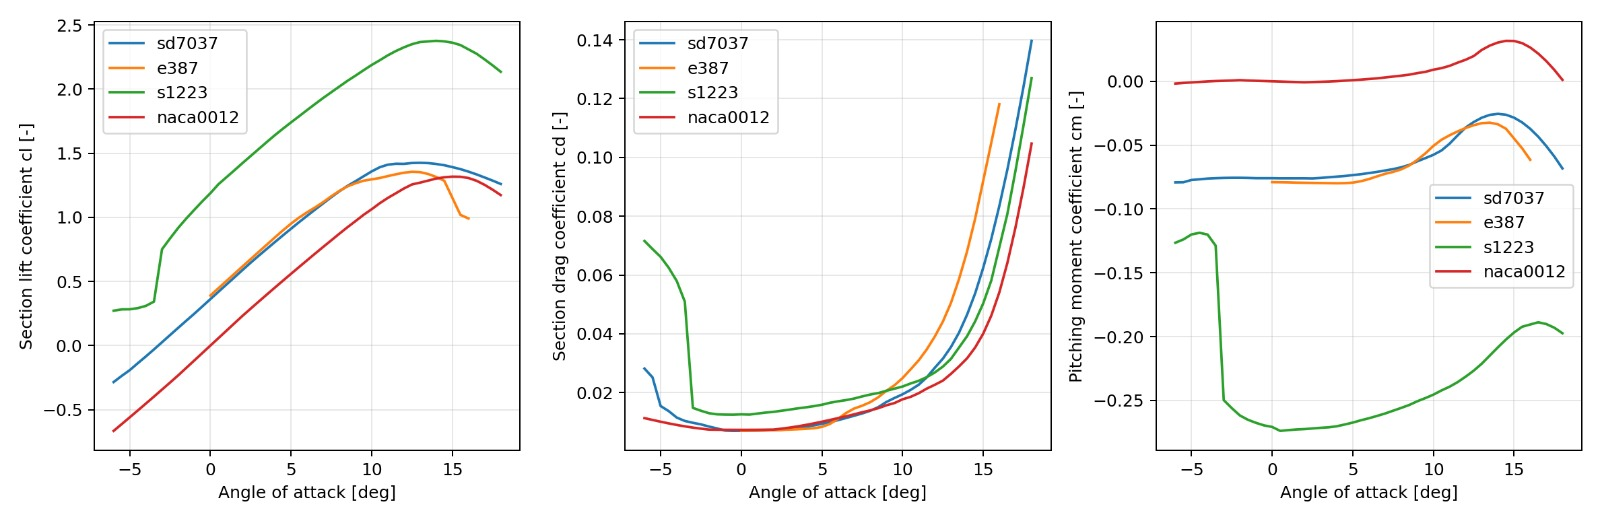
\includegraphics[width=0.9\linewidth]{figures/xf.jpeg}
    \caption{XFOIL $c_{l}-c_{d}$ curves for the selected airfoils}
    \label{fig:XFOIL}
\end{figure}
 
\begin{table}[H]
\centering
\scriptsize
\caption{Preliminary XFOIL airfoil comparison at \(Re=7.88\times10^5\) and
         \(M=0.063\).}
\label{tab:ppa_xfoil_airfoil_comparison}
\begin{tabularx}{\textwidth}{l c c c c c X}
\toprule
\textbf{Airfoil}
    & \(\boldsymbol{c_{l,\max}}\)
    & \(\boldsymbol{c_d}\) at design \(c_l\)
    & \(\boldsymbol{c_l/c_d}\)
    & \(\boldsymbol{c_{m0}}\)
    & \(\boldsymbol{c_m}\) at design \(c_l\)
    & \textbf{Implication} \\
\midrule
SD7037  & 1.426 & 0.00724 & 81.5 & -0.076 & -0.076
    & Selected main-wing section; good lift margin and low drag. \\
E387    & 1.356 & 0.00717 & 78.3 & -0.079 & -0.079
    & Efficient, with lower lift margin than SD7037. \\
S1223   & 2.377 & 0.01384 & 60.4 & -0.127 & -0.253
    & High lift, with larger drag and larger trim demand. \\
NACA~0012 & 1.318 & 0.00775 & 37.2 & 0.000 & -0.001
    & Symmetric reference for stabilising/control surfaces. \\
\bottomrule
\end{tabularx}
\end{table}
 
SD7037 is selected as the preliminary main-wing airfoil because it gives
sufficient lift margin at the design Reynolds number while keeping the drag
estimate low near the cruise lift range and maintaining a moderate
pitching-moment coefficient \cite{SeligUIUCVol2, SeligUIUCVol3}. S1223
provides the highest lift coefficient, but its higher drag and more negative
\(c_m\) at the design lift coefficient increase the canard trim demand, making
it less suitable for the selected canard tail-sitter baseline
\cite{SeligGuglielmo1997}. E387 remains a useful low-drag comparison case
\cite{McGhee1988NASA}. NACA~0012 is retained for control-surface and
stabilising-surface studies \cite{AbbottVonDoenhoff1959}.

The canard is sized after the main wing as a preliminary stabilising and
transition-control surface. A first-cut area ratio of $S_c/S_w = 0.15$,
consistent with canard tail-sitter precedent \cite{Stone1999, Raymer2018},
and a provisional moment arm of $l_c = 2.5\bar{c}_w = 2.38~\mathrm{m}$,
pending CG iteration, give a canard volume ratio
of $\bar{V}_c = S_c l_c / (S_w \bar{c}_w) = 0.38$, which falls within the
$0.3$--$0.6$ range for a destabilising canard \cite{Raymer2018,
Roskam1985PartVI}. An aspect ratio of $AR_c = 5$, lower than the main wing
to limit tip-vortex interference \cite{Raymer2018,
Roskam1985PartVI}, yields $S_c = 0.95~\mathrm{m^2}$, $b_c = 2.18~\mathrm{m}$, and $\bar{c}_c = 0.44~\mathrm{m}$. At $6000~\mathrm{m}$ cruise the canard
Reynolds number is $3.61\times10^5$, and the DATCOM formula
\cite{Polhamus1958, USAFDATCOM1978} gives $C_{L_\alpha,c} =
4.25~\mathrm{rad^{-1}}$. The three-dimensional maximum lift coefficient is
$C_{L,\max,c} = 0.9\,c_{l,\max,\text{NACA\,0012}} = 1.19$. These values
provide an initial geometry for trim, transition-control, and
structural-interface studies; the final canard incidence, elevator sizing,
and load sharing with the main wing require a longitudinal stability analysis
that accounts for canard downwash effects.
  
 
\subsubsection{Sizing results and design implications}
 
\begin{table}[H]
\centering
\scriptsize
\caption{Preliminary PPA sizing outputs for the selected canard tail-sitter baseline.}
\label{tab:ppa_preliminary_sizing_outputs}
\begin{tabularx}{0.94\textwidth}{l c X}
\toprule
\textbf{Quantity} & \textbf{Value} & \textbf{Design use} \\
\midrule
MTOW estimate          & \(50.0~\mathrm{kg}\)          & Mass baseline. \\
Wing area              & \(6.35~\mathrm{m^2}\)          & Aerodynamic and structural reference area. \\
Wing loading           & \(77.2~\mathrm{N/m^2}\)       & Constraint-diagram design point. \\
Stall \(W/S\) limit at \(6000~\mathrm{m}\) & \(96.5~\mathrm{N/m^2}\) & Stall margin check. \\
Wing span              & \(6.67~\mathrm{m}\)           & Transport and spar-layout driver. \\
Mean chord             & \(0.95~\mathrm{m}\)           & Reynolds number and control-surface input. \\
\(C_{L_\alpha}\), \(C_{L,\max,3D}\) & \(4.75~\mathrm{rad^{-1}}\), \(1.28\)
                                    & Control and stall modelling. \\
Canard area            & \(0.95~\mathrm{m^2}\)          & Preliminary trim and transition-control surface. \\
Canard span            & \(2.18~\mathrm{m}\)            & Packaging and control-authority input. \\
Canard volume ratio    & \(0.38\)                       & Preliminary longitudinal-stability sizing metric. \\
Cruise, climb, hover power & \(1.57\), \(9.21\), \(14.20~\mathrm{kW}\)
                            & Propulsion and thermal sizing. \\
Required shaft power   & \(12.14~\mathrm{kW}\)          & Motor and propeller matching. \\
Baseline battery capacity & \(3.28~\mathrm{kWh}\)      & Initial energy allocation from \autoref{tab:SpecsA}. \\
\bottomrule
\end{tabularx}
\end{table}
 
The active sizing constraint is hover at the \(6000~\mathrm{m}\) design
condition \cite{Leishman2006, Tyan2017}. Cruise power is comparatively low
because the vehicle is wing-borne in forward flight \cite{Ruijgrok2009}, while
climb and hover set the installed propulsion scale. The \(T/W=1.30\) design
point illustrated in \autoref{fig:dp}, selected to exceed Stone's \(T/W \geq 1.15\) transition floor
\cite{StoneClarke2001}, gives \(14.20~\mathrm{kW}\) electrical hover power,
above the \(9.21~\mathrm{kW}\) climb estimate. With four rotors, this
implies approximately \(3.55~\mathrm{kW}\) electrical power, or
\(3.04~\mathrm{kW}\) shaft power, per motor before transient and thermal
margins are added. The \(0.93~\mathrm{m}\) rotor diameter sets the initial
propeller packaging and tip-clearance constraint.

\begin{figure}[H]
    \centering
    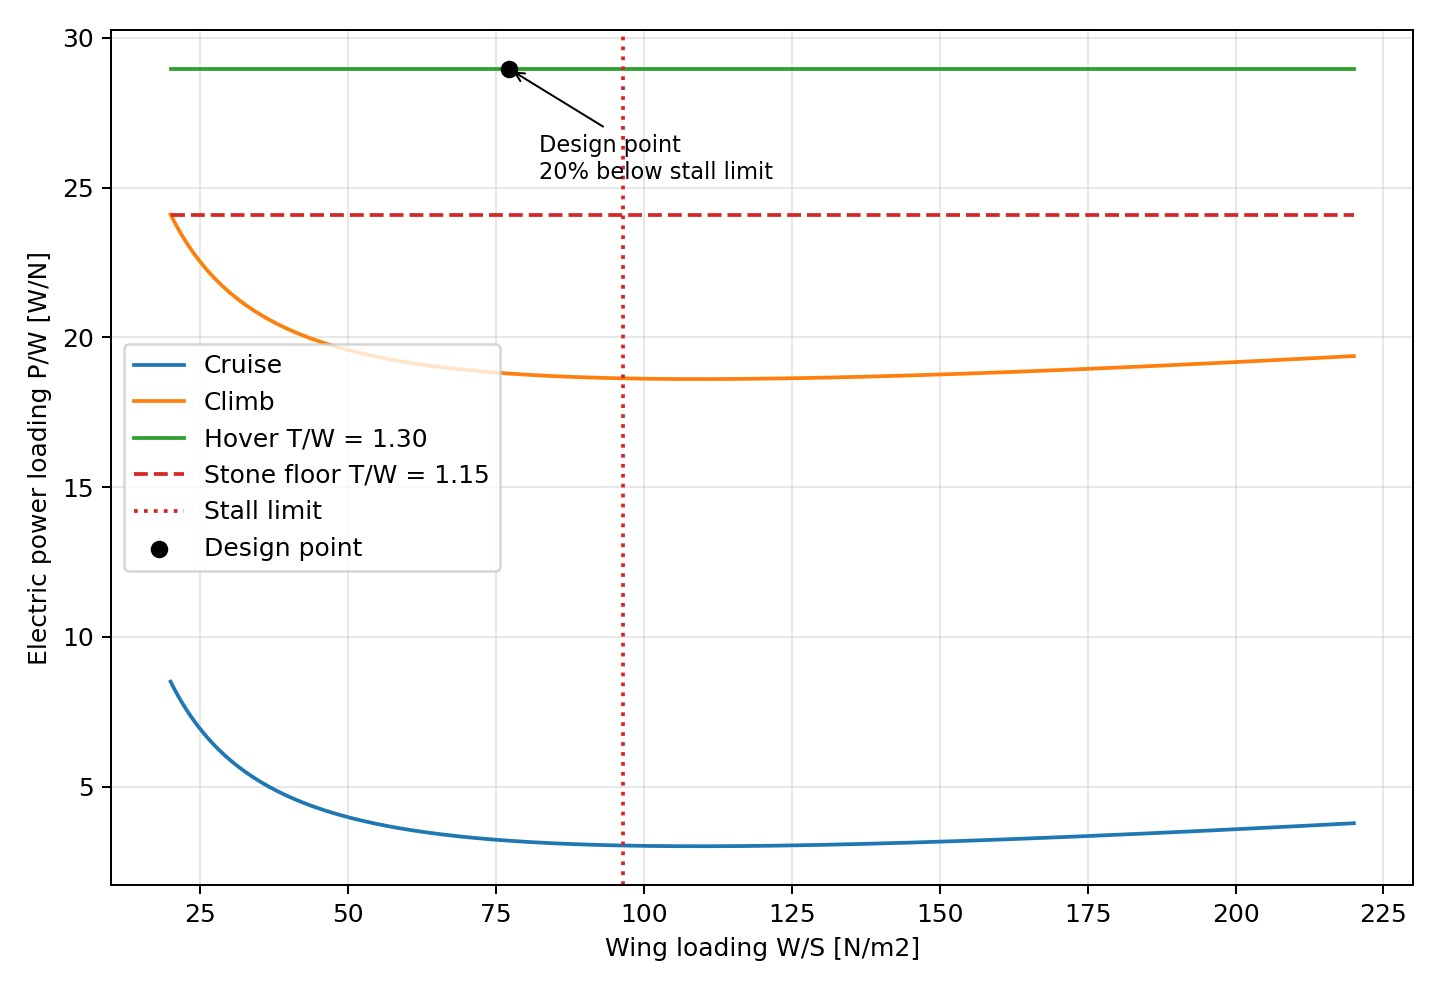
\includegraphics[width=0.5\linewidth]{figures/dp.jpeg}
    \caption{Power Loading as a function of wing loading for different phases}
    \label{fig:dp}
\end{figure}
 
The \(3.28~\mathrm{kWh}\) battery allocation remains an interim value \cite{Tyan2017}.
A full energy closure must include vertical take-off, transition, climb,
outbound cruise, terminal hover, tow, descent, avionics, reserve, and battery
discharge limits. The current results therefore support the selected canard
tail-sitter baseline, while leaving transition dynamics, propeller slipstream
effects, canard and elevon authority, roughness sensitivity, and post-capture
towing power as the main PPA uncertainties for the next design loop.

\section{Sensing, Control and Electronics}

\subsection{Sensors and stages}
The sensing suite is designed as staged pipeline aiming to reduce uncertainty by progressively introducing and trading modalities. The Sensor selection is split into the essential sensors for flight and general navigation and those for tracking. The essentials for flight are illustrated in \autoref{tab:essential_sensors}.

\begin{table}[H]
\centering
\caption{Essential Navigation, Stabilisation, and Fusion Sensors}
\label{tab:essential_sensors}
\small
\begin{tabular}{p{4cm} p{11cm}}
\toprule
\textbf{Sensor} & \textbf{Role / Function} \\ \midrule

IMU (Inertial Measurement Unit) 
&Attitude and angular velocity estimation; stabilises visual/radar tracking and enables autonomy during brief sensor dropouts. \\ 

GNSS (GPS etc.) 
& Global position reference for mid-level navigation and drift correction; provides absolute localization anchor for sensor fusion. \\ 

Barometer 
& Low-altitude vertical stability; improves relative height estimation when GNSS altitude is noisy or delayed. \\ 


\bottomrule
\end{tabular}
\end{table}


All tracking modalities considered are illustrated in \autoref{fig:DOT_sensing_ee}


\begin{figure}[H]
    \centering
    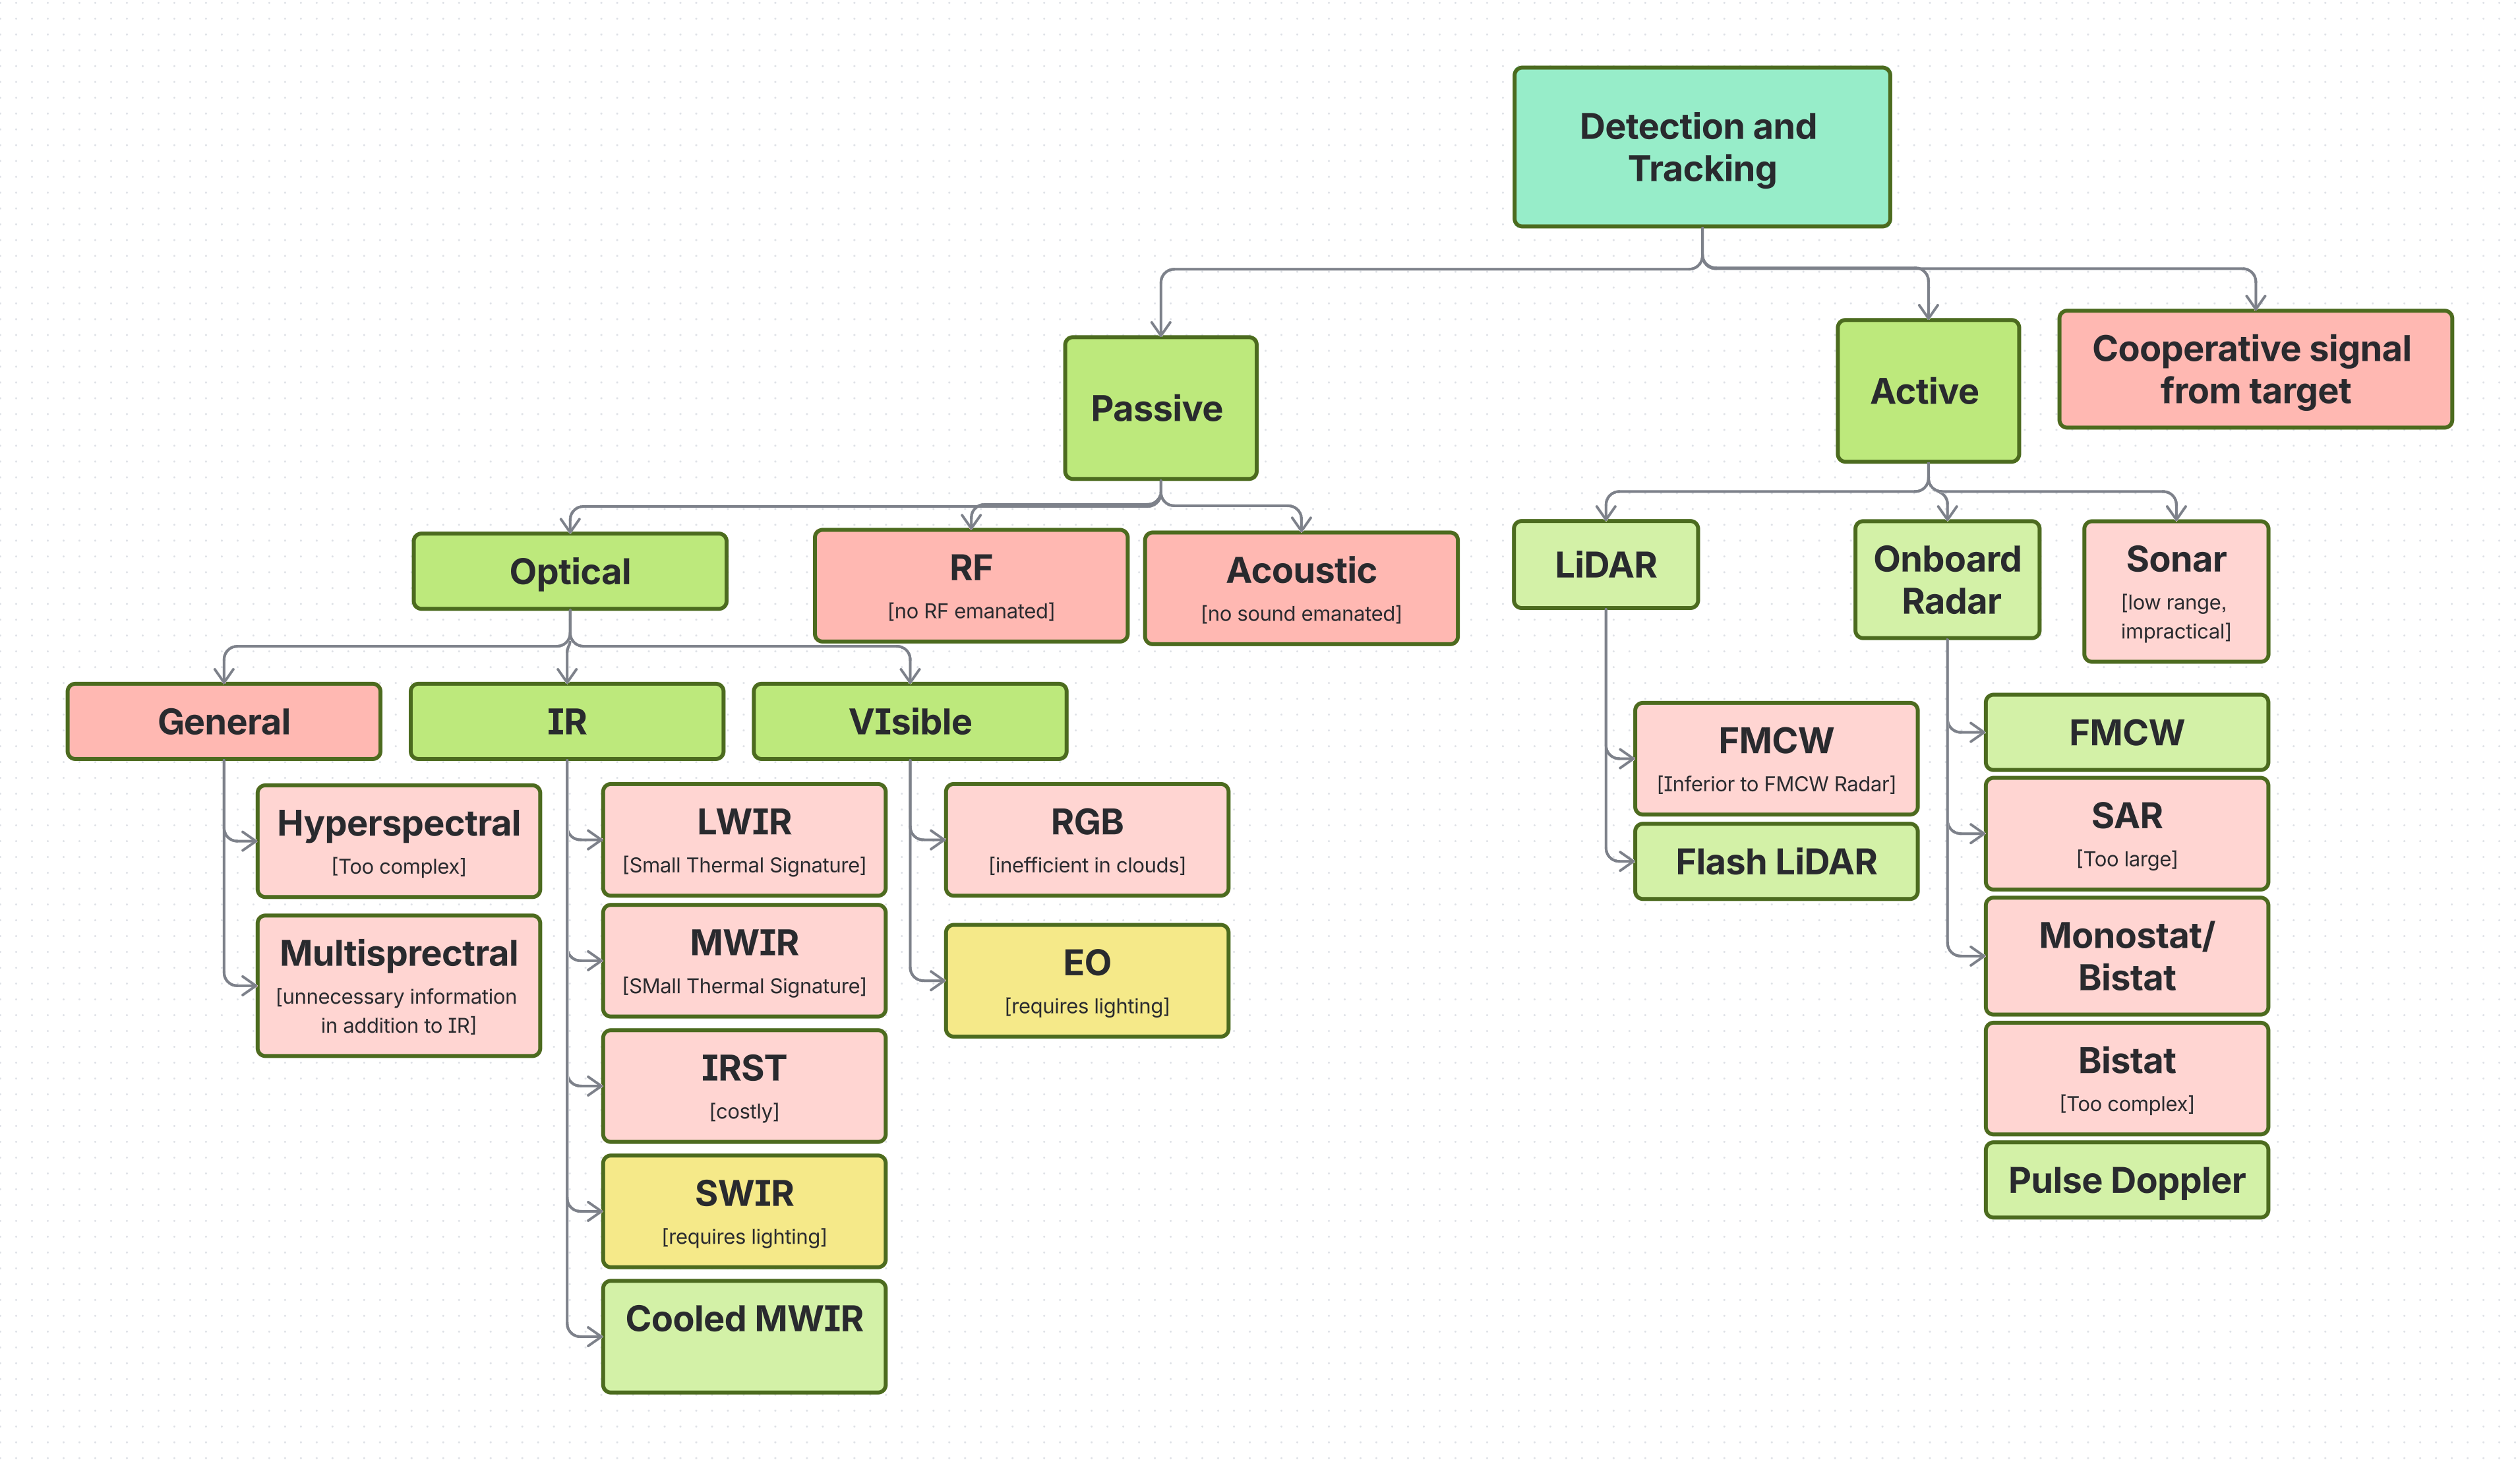
\includegraphics[width=0.75\linewidth]{figures/DOT_Sensing.png}
    \caption{DOT for Detection and Tracking}
    \label{fig:DOT_sensing_ee}
\end{figure}

The mission is decomposed into four sensing-relevant stages with distinct observability requirements and sensor roles, as shown in \autoref{tab:uav_mission_stages_sensors}. The ground based radar provides ceuing with a defined uncertinaty of 150m in range, 700m vertical and 200m width. This resutls in a worst case detection distance as shown in 

\begin{equation}
    \sqrt{(200m)^2 + (700m)^2 + (150m)^2} \approx 743m
\end{equation}



% Colour definitions
\definecolor{scoreExc}{RGB}{192,221,151}   % green  – 5 Excellent
\definecolor{scoreGood}{RGB}{181,212,244}  % blue   – 4 Good
\definecolor{scoreFair}{RGB}{250,199,117}  % amber  – 3 Fair
\definecolor{scorePoor}{RGB}{252,165,165}  % red-lite – 2 Poor
\definecolor{scoreUnacc}{RGB}{240,149,149} % red    – 1 Unacceptable
\definecolor{gateOK}{RGB}{192,221,151}     % gate passed
\definecolor{gateBlock}{RGB}{240,149,149}  % gate failed (physically infeasible)
\definecolor{stageWin}{RGB}{255,230,100}   % stage winner highlight



\begin{table}[H]
\centering
\caption{UAV Interception Mission Stages and Candidate Sensors
         (worst-case: night, OVC, uncooperative balloon \(\Delta T \approx 0.3\)–\(1\,\)K).}
\label{tab:uav_mission_stages_sensors}
\small
\begin{tabularx}{\textwidth}{p{2.5cm} p{1.6cm} X p{5.8cm}}
\toprule
\textbf{Stage} & \textbf{Range} & \textbf{Candidate Sensors} & \textbf{Primary Challenges \& Drivers} \\
\midrule

\textbf{Ground-Based Radar Transit}
  & 8.5\,km-743\,m
  & Ground-Based Radar
  & Large positional uncertainty, small balloon RCS, limited vertical resolution. \\[4pt]



\textbf{Mid-Range Tracking}
  & 743\,km–100\,m
  & FMCW Radar;\
    Cooled MWIR Camera;
    SWIR + NIR illuminator;
    Pulse-Doppler Radar (handover)
  & track continuity; wind-driven
    trajectory perturbations; clouded; low balloon RCS marginal
    thermal contrast ($\Delta T \approx 0.3\,\text{K}$). \\[4pt]

\textbf{Terminal Rel.\ Nav.}
  & 100–0\,m
  & FMCW Radar;
    Flash LiDAR;
    SWIR Camera + NIR illuminator
  & precise pose estimation ($\leq\!5\,\text{cm}$);
    low-latency; geometric constraints. \\

\bottomrule
\end{tabularx}
\end{table}

\iffalse

\begin{table}[H]
\centering
\caption{Sensors Considered but Excluded from the Trade-Off Matrix.}
\label{tab:neglected_sensors}
\small
\begin{tabularx}{\textwidth}{l X}
\toprule
\textbf{Sensor} & \textbf{Reason for Exclusion} \\
\midrule

Visible EO camera (unaided)
  & Zero passive signal at night; even with active NIR illumination
    range is limited to $\lesssim\!150\,\text{m}$ due to cloud
    backscatter, making it infeasible for Stages 1–2. Retained only
    as a possible daytime/fair-weather fallback. \\[3pt]

Uncooled microbolometer (LWIR)
  & NETD $\approx 30$–$50\,\text{mK}$ insufficient to resolve a
    balloon at $\Delta T \approx 0.3\,\text{K}$ with adequate SNR
    ($\text{SNR} < 5$ at $> 200\,\text{m}$). Cooled MWIR
    (NETD $\leq 20\,\text{mK}$) required. \\[3pt]

Multispectral imager
  & Provides spectral band differentiation useful for material
    classification in daylight; negligible advantage at night where
    all passive optical bands are signal-starved. Excluded from
    worst-case analysis. \\[3pt]

Hyperspectral imager
  & High mass ($>1\,\text{kg}$), slow frame rate ($< 10\,\text{Hz}$),
    and requires bright illumination for spectral discrimination.
    Unsuitable for a fast-closing UAV intercept geometry. \\[3pt]

Acoustic sensor
  & Rotor wash and aerodynamic noise on a UAV platform produce
    broadband noise floor 30–40\,dB above balloon acoustic signature.
    No usable SNR at standoff distances $> 10\,\text{m}$. \\[3pt]

Passive RF / ESM
  & Balloon is uncooperative and passive; no RF emissions to exploit.
    Irrelevant for this target class by definition. \\[3pt]

Passive microwave radiometry
  & Angular resolution at relevant frequencies
    ($\sim 100\,\text{GHz}$, beam $\approx 1$–$2°$) is too coarse
    to localize a $<\!1\,\text{m}$ balloon at ranges $> 100\,\text{m}$. \\[3pt]

SAR / ISAR
  & Requires significant synthetic aperture ($>10\,\text{m}$ path),
    coherent processing time incompatible with a fast intercept, and
    hardware mass $> 2\,\text{kg}$. Unsuitable for a small UAV
    interceptor platform. \\[3pt]

Single-point laser rangefinder
  & Provides 1-D range only; no angular or shape information. Useful
    as a lightweight complement for range-gating but insufficient as
    a standalone tracking or pose sensor. \\

\bottomrule
\end{tabularx}
\end{table}

\fi

\begin{table}[H]
\centering
\scriptsize
\caption{Sensor Trade-Off Matrix with Multi-Stage Weightings and Integrated Vertical Scoring (Worst-Case Scenario).}
\label{tab:sensor_multistage_inverted}

\setlength{\tabcolsep}{2pt}
\renewcommand{\arraystretch}{1.05}
\vspace{0.5ex}

\begin{tabularx}{\textwidth}{|
    >{\hsize=1.40\hsize\raggedright\arraybackslash}X|
    >{\hsize=0.80\hsize\centering\arraybackslash}X|
    >{\hsize=0.80\hsize\centering\arraybackslash}X|
    >{\hsize=0.80\hsize\centering\arraybackslash}X|
    >{\hsize=0.80\hsize\centering\arraybackslash}X|
    >{\hsize=0.80\hsize\centering\arraybackslash}X|
    >{\hsize=0.80\hsize\centering\arraybackslash}X|
}
\hline

\diagbox[
    width=\dimexpr\hsize+2\tabcolsep+2\arrayrulewidth\relax,
    height=0.065\textwidth,
    innerleftsep=1pt,
    innerrightsep=1pt
]{\textbf{\fontsize{7}{8}\selectfont Criteria}}{\textbf{\fontsize{7}{8}\selectfont Sensors}}
& \makecell[t]{\textbf{Pulse-Doppler}\\\textbf{Radar}}
& \makecell[t]{\textbf{FMCW Radar}\\\textbf{(77\,GHz)}}
& \makecell[t]{\textbf{NIR Camera}\\\textbf{(+ Illuminator)}}
& \makecell[t]{\textbf{LWIR Camera}\\\textbf{(Thermal)}}
& \makecell[t]{\textbf{SWIR Cam.}}
& \makecell[t]{\textbf{Flash}\\\textbf{LiDAR}}
\\ \hline

% ---- Cost -------------------------------------------------------
\parbox[t]{\linewidth}{\textbf{Cost}\\[0.1ex]{\fontsize{6}{7}\selectfont Weights: $[S_1{=}0.1, S_2{=}0.1]$}}
& \cellcolor{orange!40}\makecell[t]{\textbf{2}\\[-0.7ex]
    \fontsize{5}{6}\selectfont \$10k--\$40k\\[-0.7ex]
    \fontsize{5}{6}\selectfont Specialized RF\\[-0.7ex]
    \fontsize{5}{6}\selectfont \cite{Echodyne2026EchoShieldRadar}}
& \cellcolor{green!40}\makecell[t]{\textbf{5}\\[-0.7ex]
    \fontsize{5}{6}\selectfont \$50--\$500\\[-0.7ex]
    \fontsize{5}{6}\selectfont TI AWR1843:\\[-0.7ex]
    \fontsize{5}{6}\selectfont automotive \cite{TI_AWR1843}}
& \cellcolor{green!40}\makecell[t]{\textbf{5}\\[-0.7ex]
    \fontsize{5}{6}\selectfont \$50--\$200\\[-0.7ex]
    \fontsize{5}{6}\selectfont Standard CMOS\\[-0.7ex]
    \fontsize{5}{6}\selectfont Uncooled Silicon}
& \cellcolor{red!40}\makecell[t]{\textbf{1}\\[-0.7ex]
    \fontsize{5}{6}\selectfont \$40k--\$70k\\[-0.7ex]
    \fontsize{5}{6}\selectfont cooled infrared\\[-0.7ex]
    \fontsize{5}{6}\selectfont \cite{Cooled_camera}}
& \cellcolor{yellow!40}\makecell[t]{\textbf{3}\\[-0.7ex]
    \fontsize{5}{6}\selectfont \$1k--\$3k\\[-0.7ex]
    \fontsize{5}{6}\selectfont InGaAs cam.\\[-0.7ex]
    \fontsize{5}{6}\selectfont + NIR \cite{Driggers2012}}
& \cellcolor{yellow!40}\makecell[t]{\textbf{3}\\[-0.7ex]
    \fontsize{5}{6}\selectfont \$1k\\[-0.7ex]
    \fontsize{5}{6}\selectfont Hesai FTX\\[-0.7ex]
    \fontsize{5}{6}\selectfont \cite{hesai_flash_lidar}}
\\ \hline

% ---- Detection Range --------------------------------------------
\parbox[t]{\linewidth}{\textbf{Detection Range}\\[0.1ex]{\fontsize{6}{7}\selectfont Weights: $[S_1{=}0.2, S_2{=}0.0]$}}
& \cellcolor{blue!30}\makecell[t]{\textbf{4}\\[-0.7ex]
    \fontsize{5}{6}\selectfont 1--3\,km\\[-0.7ex]
    \fontsize{5}{6}\selectfont $P_t$=1--10\,kW;\\[-0.7ex]
    \fontsize{5}{6}\selectfont $\sigma$=0.01\,m$^2$ \cite{Richards2010}}
& \cellcolor{orange!40}\makecell[t]{\textbf{2}\\[-0.7ex]
    \fontsize{5}{6}\selectfont 10--300\,m\\[-0.7ex]
    \fontsize{5}{6}\selectfont EIRP-limit;\\[-0.7ex]
    \fontsize{5}{6}\selectfont low RCS \cite{Soumya2023RecentReview}}
& \cellcolor{orange!40}\makecell[t]{\textbf{2}\\[-0.7ex]
    \fontsize{5}{6}\selectfont 10--300\,m\\[-0.7ex]
    \fontsize{5}{6}\selectfont Ambient light\\[-0.7ex]
    \fontsize{5}{6}\selectfont dependent}
& \cellcolor{yellow!40}\makecell[t]{\textbf{3}\\[-0.7ex]
    \fontsize{5}{6}\selectfont 400--800\,m\\[-0.7ex]
    \fontsize{5}{6}\selectfont $\Delta T$=0.3\,K \cite{Vollmer2018}}
& \cellcolor{orange!40}\makecell[t]{\textbf{2}\\[-0.7ex]
    \fontsize{5}{6}\selectfont 50--200\,m\\[-0.7ex]
    \fontsize{5}{6}\selectfont Cloud scatter\\[-0.7ex]
    \fontsize{5}{6}\selectfont caps range \cite{Driggers2012}}
& \cellcolor{red!40}\makecell[t]{\textbf{1}\\[-0.7ex]
    \fontsize{5}{6}\selectfont $<$50\,m\\[-0.7ex]
    \fontsize{5}{6}\selectfont $1/R^4$ + aeros.}
\\ \hline

% ---- Pose Accuracy ----------------------------------------------
\parbox[t]{\linewidth}{\textbf{Pose Accuracy}\\[0.1ex]{\fontsize{6}{7}\selectfont Weights: $[S_1{=}0.2, S_2{=}0.5]$}}
& \cellcolor{red!40}\makecell[t]{\textbf{1}\\[-0.7ex]
    \fontsize{5}{6}\selectfont Rng: $\pm$1--5\,m\\[-0.7ex]
    \fontsize{5}{6}\selectfont Brg: $\pm$2--5$^{\circ}$\\[-0.7ex]
    \fontsize{5}{6}\selectfont poor close \cite{Stimson1998}}
& \cellcolor{blue!30}\makecell[t]{\textbf{4}\\[-0.7ex]
    \fontsize{5}{6}\selectfont Rng: $\pm$5--20\,cm\\[-0.7ex]
    \fontsize{5}{6}\selectfont Vel: $\pm$0.05\,m/s\\[-0.7ex]
    \fontsize{5}{6}\selectfont Az: $\pm$0.5--2$^{\circ}$ \cite{TI_AWR1843}}
& \cellcolor{blue!30}\makecell[t]{\textbf{4}\\[-0.7ex]
    \fontsize{5}{6}\selectfont High Res PnP\\[-0.7ex]
    \fontsize{5}{6}\selectfont $\pm$1--3\,cm@10m\\[-0.7ex]
    \fontsize{5}{6}\selectfont Az: $\pm$0.02$^{\circ}$}
& \cellcolor{yellow!40}\makecell[t]{\textbf{3}\\[-0.7ex]
    \fontsize{5}{6}\selectfont Brg: $\pm$0.1--0.3$^{\circ}$\\[-0.7ex]
    \fontsize{5}{6}\selectfont Thermal blur\\[-0.7ex]
    \fontsize{5}{6}\selectfont SNR $\approx$ 5 \cite{Vollmer2018}}
& \cellcolor{blue!30}\makecell[t]{\textbf{4}\\[-0.7ex]
    \fontsize{5}{6}\selectfont PnP pose:\\[-0.7ex]
    \fontsize{5}{6}\selectfont $\pm$2--5\,cm@10m\\[-0.7ex]
    \fontsize{5}{6}\selectfont Az: $\pm$0.05$^{\circ}$}
& \cellcolor{green!40}\makecell[t]{\textbf{5}\\[-0.7ex]
    \fontsize{5}{6}\selectfont 3-D: $\pm$2--5\,cm\\[-0.7ex]
    \fontsize{5}{6}\selectfont $>$1M pts/s\\[-0.7ex]
    \fontsize{5}{6}\selectfont Az: $\pm$0.1$^{\circ}$ \cite{Raj2020}}
\\ \hline

% ---- Environmental Robustness -----------------------------------
\parbox[t]{\linewidth}{\textbf{Env. Robustness}\\[0.1ex]{\fontsize{6}{7}\selectfont Weights: $[S_1{=}0.2, S_2{=}0.2]$}}
& \cellcolor{green!40}\makecell[t]{\textbf{5}\\[-0.7ex]
    \fontsize{5}{6}\selectfont RF loss $<$0.5dB\\[-0.7ex]
    \fontsize{5}{6}\selectfont per km rain; MTI\\[-0.7ex]
    \fontsize{5}{6}\selectfont filter \cite{Richards2010}}
& \cellcolor{green!40}\makecell[t]{\textbf{5}\\[-0.7ex]
    \fontsize{5}{6}\selectfont Fog: $<$0.2\,dB\\[-0.7ex]
    \fontsize{5}{6}\selectfont per km; Doppler\\[-0.7ex]
    \fontsize{5}{6}\selectfont reject \cite{TI_AWR1843}}
& \cellcolor{orange!40}\makecell[t]{\textbf{2}\\[-0.7ex]
    \fontsize{5}{6}\selectfont Severe Mie scatter\\[-0.7ex]}
& \cellcolor{orange!40}\makecell[t]{\textbf{2}\\[-0.7ex]
    \fontsize{5}{6}\selectfont LWIR opaque\\[-0.7ex]
    \fontsize{5}{6}\selectfont to OVC cloud;\\[-0.7ex]
    \fontsize{5}{6}\selectfont $\Delta T$ limit \cite{Vollmer2018}}
& \cellcolor{yellow!40}\makecell[t]{\textbf{3}\\[-0.7ex]
    \fontsize{5}{6}\selectfont Cloud backscat\\[-0.7ex]
    \fontsize{5}{6}\selectfont +8--12\,dB;\\[-0.7ex]
    \fontsize{5}{6}\selectfont halved \cite{Driggers2012}}
& \cellcolor{red!40}\makecell[t]{\textbf{1}\\[-0.7ex]
    \fontsize{5}{6}\selectfont OVC: range\\[-0.7ex]
    \fontsize{5}{6}\selectfont $<$50\,m; aerosol\\[-0.7ex]
    \fontsize{5}{6}\selectfont saturat.}
\\ \hline

% ---- Angular Wideness -------------------------------------------
\parbox[t]{\linewidth}{\textbf{Angular Wideness}\\[0.1ex]{\fontsize{6}{7}\selectfont Weights: $[S_1{=}0.2, S_2{=}0.1]$}}
& \cellcolor{yellow!40}\makecell[t]{\textbf{3}\\[-0.7ex]
    \fontsize{5}{6}\selectfont Mech $\pm$60$^{\circ}$ azimuth\\[-0.7ex]
    \fontsize{5}{6}\selectfont elevation $\pm$15$^{\circ}$;\\[-0.7ex]
    \fontsize{5}{6}\selectfont 1--2\,Hz}
& \cellcolor{orange!40}\makecell[t]{\textbf{2}\\[-0.7ex]
    \fontsize{5}{6}\selectfont Phase $\pm$45$^{\circ}$ azimuth\\[-0.7ex]
    \fontsize{5}{6}\selectfont elevation $\pm$15$^{\circ}$;\\[-0.7ex]
    \fontsize{5}{6}\selectfont beam 2-5$^{\circ}$ \cite{TI_AWR1843}}
& \cellcolor{blue!30}\makecell[t]{\textbf{4}\\[-0.7ex]
    \fontsize{5}{6}\selectfont Wide FOV avail.\\[-0.7ex]
    \fontsize{5}{6}\selectfont 60--110$^{\circ}$ optics\\[-0.7ex]
    \fontsize{5}{6}\selectfont High res array}
& \cellcolor{yellow!40}\makecell[t]{\textbf{3}\\[-0.7ex]
    \fontsize{5}{6}\selectfont FOV 25--45$^{\circ}$\\[-0.7ex]
    \fontsize{5}{6}\selectfont gimbal steer;\\[-0.7ex]
    \fontsize{5}{6}\selectfont no scan}
& \cellcolor{blue!30}\makecell[t]{\textbf{4}\\[-0.7ex]
    \fontsize{5}{6}\selectfont FOV 60--90$^{\circ}$\\[-0.7ex]
    \fontsize{5}{6}\selectfont illum. cone\\[-0.7ex]
    \fontsize{5}{6}\selectfont $\approx$20$^{\circ}$ eff. \cite{Driggers2012}}
& \cellcolor{orange!40}\makecell[t]{\textbf{2}\\[-0.7ex]
    \fontsize{5}{6}\selectfont FOV 10--20$^{\circ}$;\\[-0.7ex]
    \fontsize{5}{6}\selectfont staring aperture\\[-0.7ex]
    \fontsize{5}{6}\selectfont no scan \cite{Raj2020}}
\\ \hline

% ---- Weight -----------------------------------------------------
\parbox[t]{\linewidth}{\textbf{Weight}\\[0.1ex]{\fontsize{6}{7}\selectfont Weights: $[S_1{=}0.1, S_2{=}0.1]$}}
& \cellcolor{orange!40}\makecell[t]{\textbf{2}\\[-0.7ex]
    \fontsize{5}{6}\selectfont 800g--15kg\\[-0.7ex]
    \fontsize{5}{6}\selectfont heavy RF \cite{Skolnik2001IntroductionSystems}}
& \cellcolor{green!40}\makecell[t]{\textbf{5}\\[-0.7ex]
    \fontsize{5}{6}\selectfont aWR1843: 12\,g\\[-0.7ex]
    \fontsize{5}{6}\selectfont 1--3\,W; PCB\\[-0.7ex]
    \fontsize{5}{6}\selectfont integ. \cite{TI_AWR1843}}
& \cellcolor{green!40}\makecell[t]{\textbf{5}\\[-0.7ex]
    \fontsize{5}{6}\selectfont 15--50\,g\\[-0.7ex]
    \fontsize{5}{6}\selectfont $<$1.5\,W power\\[-0.7ex]
    \fontsize{5}{6}\selectfont Ultra-lightweight}
& \cellcolor{red!40}\makecell[t]{\textbf{1}\\[-0.7ex]
    \fontsize{5}{6}\selectfont 0.8--4kg Stirling\\[-0.7ex]
    \fontsize{5}{6}\selectfont cooler 6--20W\\[-0.7ex]
    \fontsize{5}{6}\selectfont heavy UAV}
& \cellcolor{green!40}\makecell[t]{\textbf{5}\\[-0.7ex]
    \fontsize{5}{6}\selectfont 150--400g tot\\[-0.7ex]
    \fontsize{5}{6}\selectfont InGaAs+laser\\[-0.7ex]
    \fontsize{5}{6}\selectfont 5--15W \cite{Driggers2012}}
& \cellcolor{yellow!40}\makecell[t]{\textbf{3}\\[-0.7ex]
    \fontsize{5}{6}\selectfont 250\,g \cite{Ouster2023}\\[-0.7ex]}
\\ \hline

\parbox[t]{\linewidth}{Feasibility Gate}
& \makecell[c]{ S1: \texttimes\ S2: \texttimes}
& \makecell[c]{ S1: \checkmark\ S2: \checkmark}
& \makecell[c]{ S1: \checkmark\ S2: \checkmark}
& \makecell[c]{ S1: \texttimes\ S2: \texttimes}
& \makecell[c]{ S1: \checkmark\ S2: \checkmark}
& \makecell[c]{ S1: \texttimes\ S2: \checkmark}
\\ \hline

Stage 1 Score (Tracking)    & 0.00 & 3.80 & 3.40 & 0.00 & 3.40 & 0.00 \\ \hline
Stage 2 Score (Terminal Nav)& 0.00 & 4.20 & 3.80 & 0.00 & 3.80 & 3.50 \\ \hline

\end{tabularx}
\end{table}

This trade-off highlights a stark detection-and-budget gap. Specifically, a range of up to 740~m is unserviceable within budget, as Pulse-Doppler radars cost upwards of \$10k; consequently, search maneuvers will be incorporated along the Line of Sight (LOS) of the ground-based radar.


This trade-off then leads to a preliminary sensor stack, structured to balance continuous observability across all mission stages and development constraints.The resulting stack is as follows: \textbf{(i)} an inertial/GNSS/barometer core for state estimation and stability across all phases; \textbf{(ii)} an FMCW radar as the primary mid-range tracker (743~m--100~m), augmented by NIR EO system with illumination for angular refinement;  and \textbf{(iii)} a flash LiDAR system augmenting the already chosen FMCW Radar for terminal navigation (100--0~m), providing high-precision relative pose under favourable visibility.




\subsection{Communication and Ground Link}
The communication subsystem is divided into a command-and-telemetry link, a video downlink, a ground-cue upload path, and an independent manual-override link. The command-and-telemetry link carries low-bandwidth but safety-relevant data such as UAV position, attitude, battery state, and health warnings. The video downlink is separated from this link as it requires higher data rate. The manual-override link provides an independent safety path to the flight controller, allowing the operator to take control or command an abort if the autonomous mission becomes unsafe.
\subsection{Control \& Guidance Strategy}

The guidance system is structured as a probabilistic, stage-dependent control architecture driven by a state estimator and wind-aware prediction model. An Extended or Unscented Kalman Filter (EKF/UKF) is used to fuse modalities with a stochastic wind-field model, producing a continuously updated belief over target position and velocity. 

Uncertainty-aware trajectory planning reduces sensitivity to bad sensor data and wind shear discontinuities. Guidance laws are stage-dependent: energy-efficient transit dominates at long range, while information-gain-driven motion is prioritized during acquisition to reduce estimation uncertainty.


At the control layer, Incremental Nonlinear Dynamic Inversion (INDI) is preferred over classical PID control due to its improved robustness under model uncertainty, actuator nonlinearity, and rapidly varying aerodynamic conditions at altitude.



\subsection{Electronics \& Thermal Management}
The electrical architecture is divided into two complementary schematics. 
\autoref{fig:electronics_thermal} shows the avionics, sensing, control, communication, and health-management architecture. 
Sensor data are processed by the onboard computer and flight controller, which provide mission-level guidance and real-time stabilisation respectively. 
The health and thermal management block supervises subsystem temperatures and fault states, while the data logger records mission, sensor, actuator, and health data for post-flight analysis.

\autoref{fig:power_distribution} shows the electrical power distribution architecture. 
The main battery supplies the high-voltage power bus through the BMS, protection, pre-charge, and contactor stages. 
The power distribution system then supplies the ESCs and propulsion motors directly, while DC/DC converters generate lower-voltage supplies for avionics, sensors, communication, and balloon-interaction mechanisms. 
A backup low-voltage avionics battery provides emergency power to essential control and communication functions. 
Power monitoring and shutdown control provide fault detection and electrical isolation during abnormal conditions.\\
The thermal-management system uses passive heat spreading combined with propwash and duct-assisted convection. ESCs are mounted on heat sinks exposed to rotor slipstream, while DC/DC converters and actuator drivers are mounted to aluminium heat spreaders connected to side cooling ducts. Thermal pads or tapes provide the conductive interface between electronics and heat spreaders. The onboard computer receives a dedicated heat sink and optional fan. Temperature sensors on the battery, ESCs, motors, converters, and avionics bay provide input to the health-management system, which can command abort, or shutdown if thermal limits are exceeded.

\begin{figure}[H]
    \centering

    \begin{subfigure}[t]{0.48\textwidth}
        \centering
        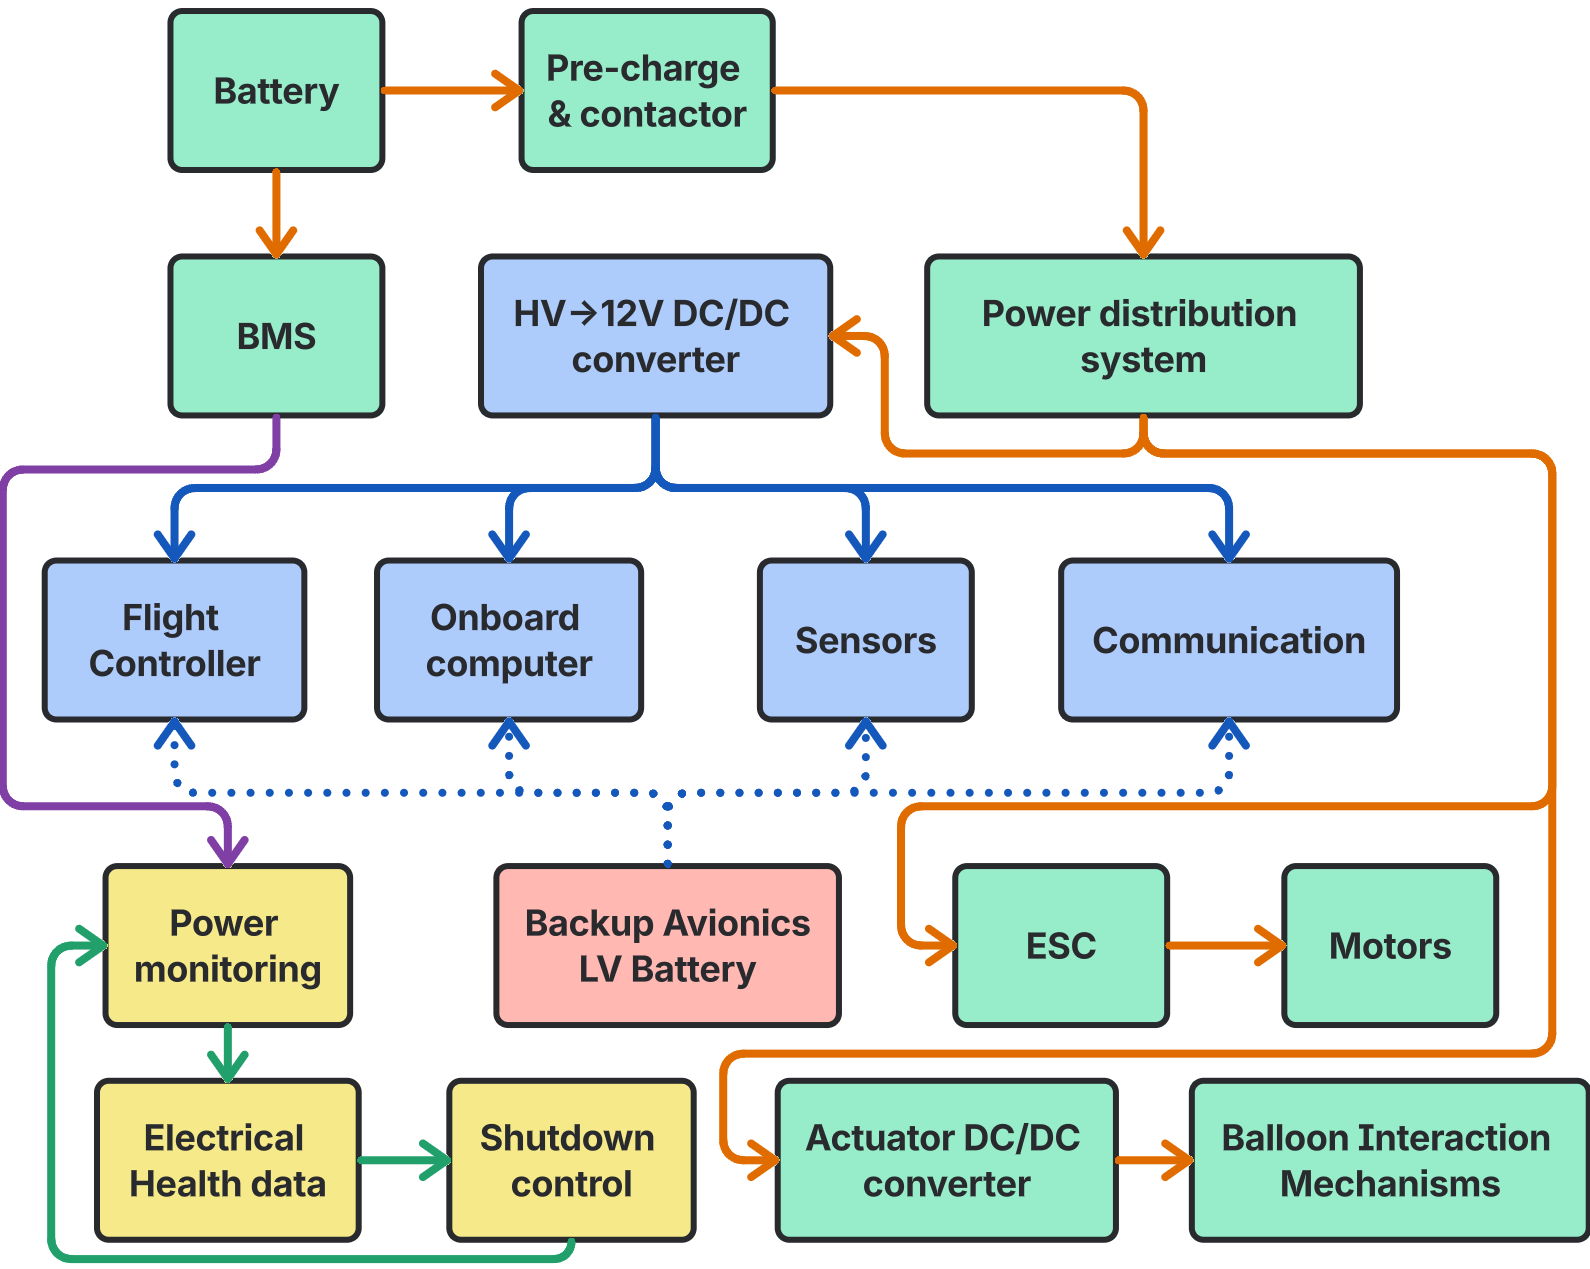
\includegraphics[width=\linewidth]{figures/Power distribution.png}
        \caption{Power distribution architecture.}
        \label{fig:power_distribution}
    \end{subfigure}
    \hfill
    \begin{subfigure}[t]{0.48\textwidth}
        \centering
        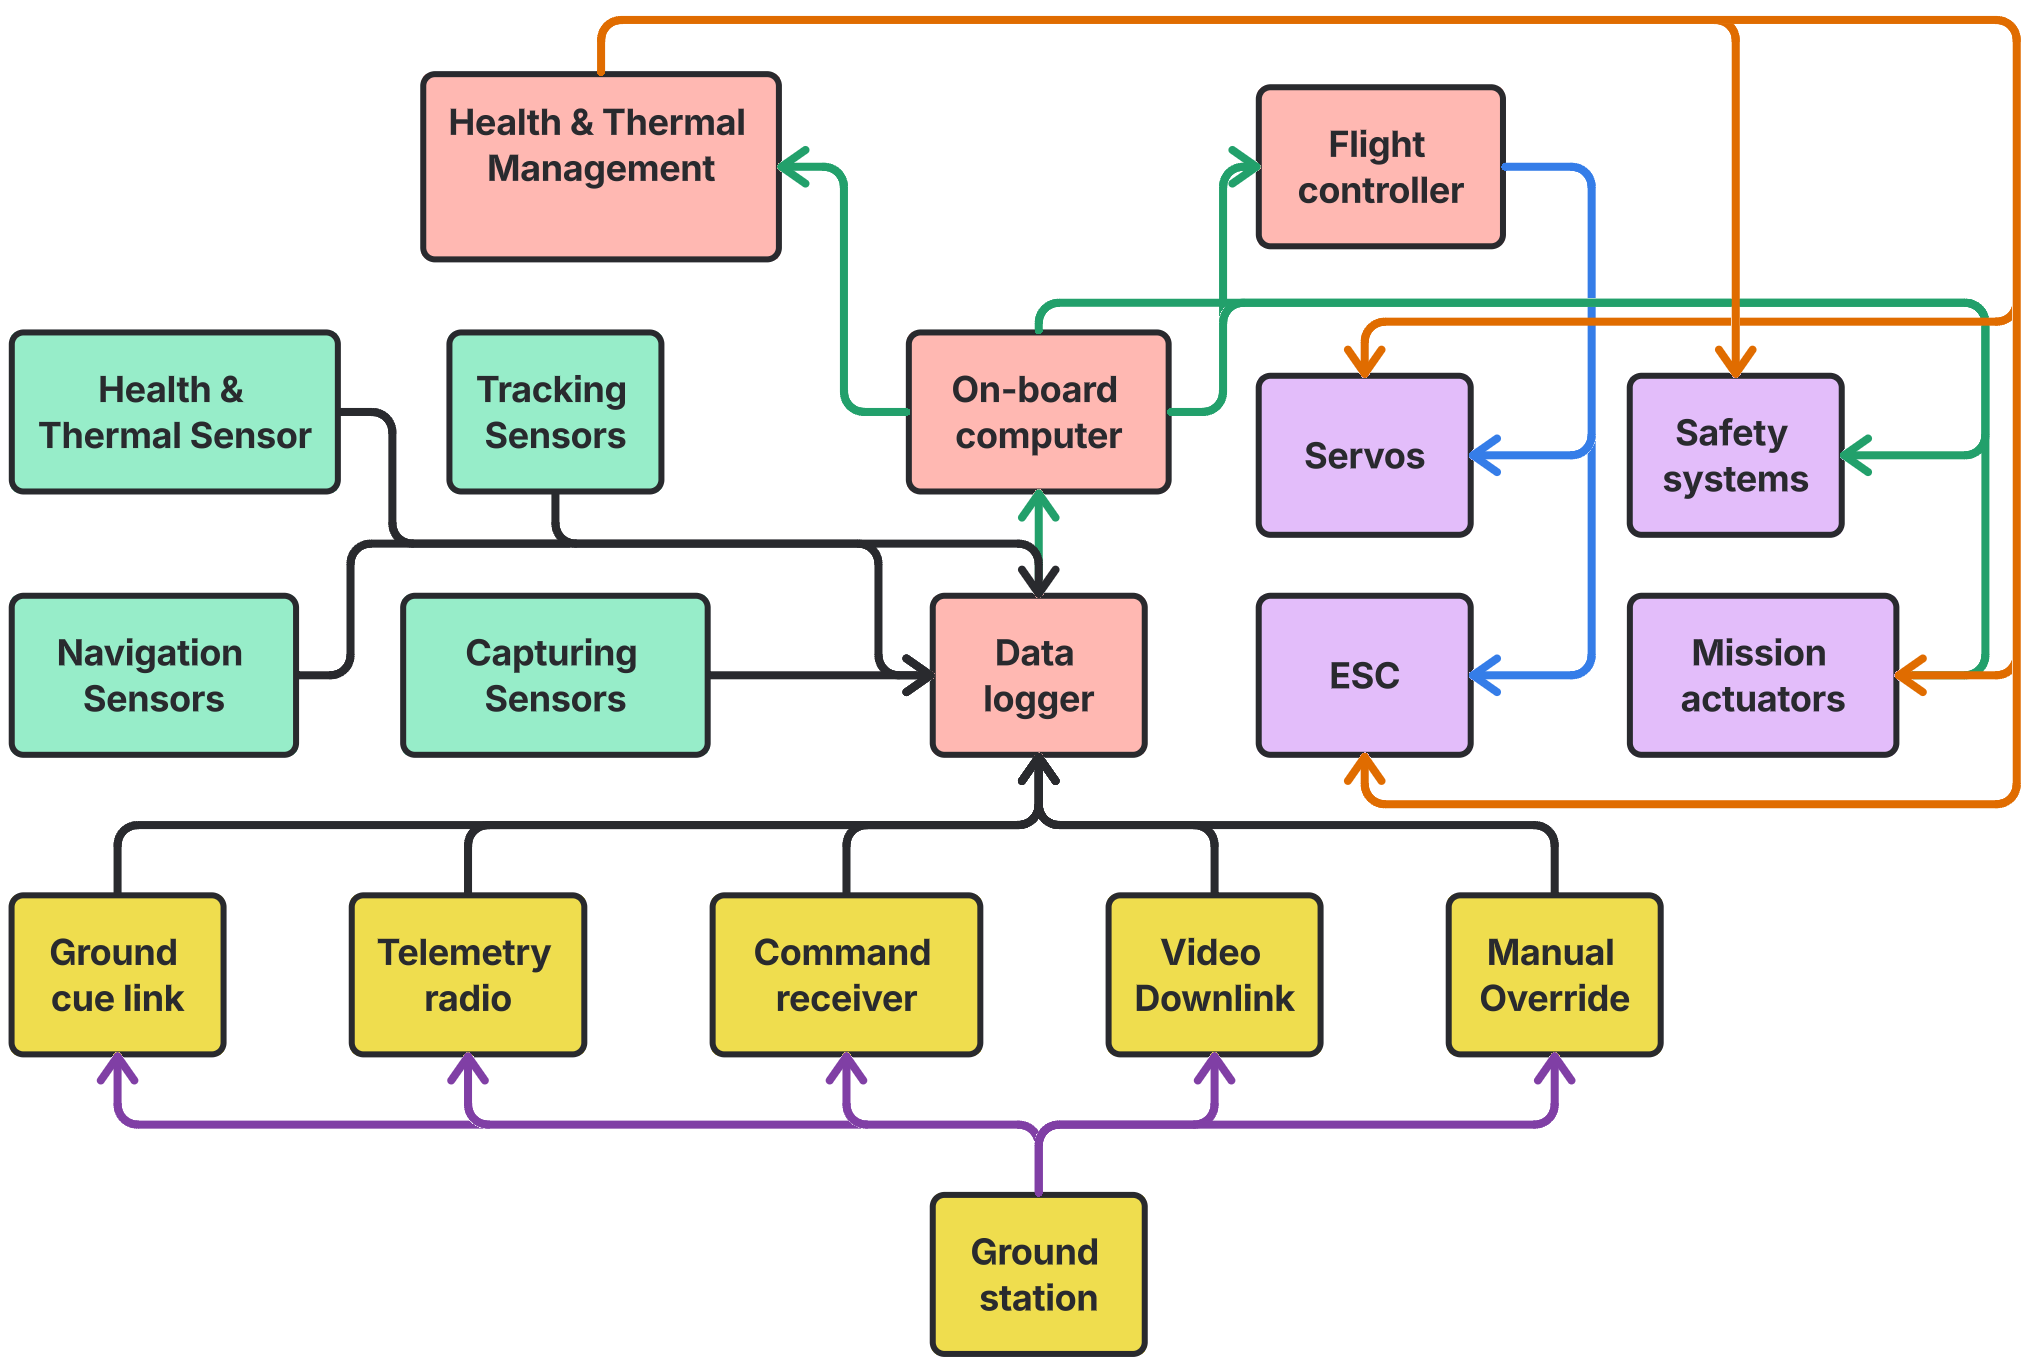
\includegraphics[width=\linewidth]{figures/Electronics.png}
        \caption{Electronics and thermal-management architecture.}
        \label{fig:electronics_thermal}
    \end{subfigure}

    \caption{Electrical system architecture, including power distribution, avionics, sensing, actuation, communication, and thermal-management interfaces.}
    \label{fig:electrical_architecture}
\end{figure}

\section{Structures, Materials and Sustainability}

The structures, materials, and sustainability analysis focuses on the airframe load paths, critical interfaces, material selection, deployment architecture, and repairability of Concept A. The UAV acts both as an aircraft and as a load-carrying recovery element after payload capture. Therefore, the structure is governed by two load paths: the conventional flight load path and the capture load path.



% The structures, materials, and sustainability analysis focuses on the airframe load paths, critical interfaces, material selection, deployment architecture, and repairability of Concept A. The UAV acts both as an aircraft and as a load-carrying recovery element after payload capture. Therefore, the structure is governed by two load paths: the conventional flight load path and the capture load path.



% The structures and materials considerations for this conceptual design are strongly linked to its balloon interaction strategy. The UAV does not only act as an aircraft, but as a load carrying element after the payload was captured. Therefore, the structural design is governed by two main loadpaths.   \\

% The first load path is the conventional flight load path, in which propulsive, aerodynamic and inertial loads are transferred through the motor mounts, wing and tail roots, fusselage and landing supports. The second is the capture load path, in which the load is transfered from the payload, to the net and then into the tether and the fuselage hardpoint. This load path is a treated as the principal structural design driver, since the failure of this interface would lead to the loss of control over the balloon-payload envelope.  \\


% % The objective at this phase is to identify the structural design drivers, define the critical load cases, select preliminary material families and identify which interfaces require a more detailed sizing during the final design phase. 

% The preliminary material allocation follows a mixed-material approach. Carbon-fibre reinforced polymer is selected for the main lightweight airframe members, such as spars, stiffeners, and fuselage panels, because the platform is mass-sensitive during climb, hover, and transition. Aluminium alloy is retained for local hardpoints, motor mounts, reel brackets, launcher brackets, and bolted interfaces because these parts experience concentrated loads and must remain inspectable and replaceable. The net and tether are based on UHMWPE or HMPE fibres, since the interaction subsystem requires high tensile strength at low mass while remaining flexible, foldable, and reusable. Non-primary fairings and sensor covers can be manufactured from lightweight polymer or composite parts, since these elements mainly provide aerodynamic shaping and protection rather than primary load carrying. look up for sources for materials now yea? 



\subsection{Structural Design Drivers}

\begin{table}[H]
\centering
\small
\caption{Main structural design drivers for Concept A.}
\label{tab:concept_a_structural_drivers}
\begin{tabularx}{\textwidth}{p{0.26\textwidth} X}
\toprule
\textbf{Driver} & \textbf{Design implication} \\
\midrule
Capture load path & Tether hardpoint, reel mount, and fuselage frame require local reinforcement and direct load transfer. \\
Removable wing modules & Wing-root joints must transfer bending, shear, torsion, motor thrust, and landing loads after repeated assembly cycles. \\
Propulsion loads & Motor mounts must resist thrust, vibration, and torque from large propellers during hover and transition. \\
Landing and handling & Landing supports and contact pads must be replaceable and protect the primary structure during recovery. \\
Mass and stiffness & Primary lifting structure must remain lightweight while providing sufficient stiffness for transition and control. \\
\bottomrule
\end{tabularx}
\end{table}% \begin{table}[H]


\subsection{Preliminary Structural Load Cases}

The main structural load cases are listed in Table~\ref{tab:concept_a_structural_load_cases}. These load cases define the first set of design drivers for the final structural sizing. The capture-related cases are expected to be the most critical because they introduce concentrated loads into the airframe and may occur while the vehicle is already operating close to its control limits. The first one is presented in \autoref{fig:lc1}. Other load cases differ depending on the configuration, as having stabilizing force placed at either tail or canard redefine the structural analysis, thus these will be visualized after the configuration is determined.
\setlength{\tabcolsep}{2pt}
\renewcommand{\arraystretch}{1.03}
\setlength{\LTpre}{2pt}
\setlength{\LTpost}{2pt}

\begin{longtable}{@{}
>{\raggedright\arraybackslash}p{0.075\textwidth}
>{\raggedright\arraybackslash}p{0.235\textwidth}
>{\raggedright\arraybackslash}p{0.655\textwidth}
@{}}
\caption{Preliminary structural load cases for the selected concept.} 
\label{tab:concept_a_structural_load_cases} \\
\toprule
\textbf{Load case} & \textbf{Description} & \textbf{Critical structural elements} \\
\midrule
\endfirsthead

\multicolumn{3}{l}{\small\textit{Table \ref{tab:concept_a_structural_load_cases} continued from previous page}} \\
\toprule
\textbf{Load case} & \textbf{Description} & \textbf{Critical structural elements} \\
\midrule
\endhead

\midrule
\multicolumn{3}{r}{\small\textit{Continued on next page}} \\
\endfoot

\bottomrule
\endlastfoot

LC1 & Hover and climb at maximum take-off mass. 
& Motor mounts, boom or wing roots, central fuselage frame, battery support, and landing supports. \\

LC2 & Transition between cruise and hover or low-speed approach. 
& Wing roots, canard attachments, fuselage torsion path, control-surface attachments, and propulsion mounts. \\

LC3 & Maximum tether or net load after capture. 
& Tether hardpoint, reel mount, central fuselage frame, load-spreading fittings, and local reinforcement around the attachment point. \\

LC4 & Landing after mission or recovery. 
& Landing supports, lower fuselage frame, battery restraint, propeller clearance zones, and payload/interaction mechanism attachment. \\

\end{longtable}


\begin{figure}[H]
    \centering
    \resizebox{0.6\textwidth}{!}{%
        \clipbox{0pt 20pt 0pt 70pt}{%
            \includestandalone{figures/LC1}
        }
    }
    \caption{Loading Diagram for Load Case 1}
    \label{fig:lc1}
\end{figure}

\subsection{Preliminary Structural Geometry and Interface Envelopes}

The main structural dimensions are summarised before defining the load cases, because the geometry determines the load paths, transportability, and subsystem packaging of Concept A. At this stage, the values are preliminary design-envelope values rather than final manufacturing dimensions. They will be refined after the aerodynamic layout, centre-of-gravity position, propulsion placement, and tether hardpoint loads are frozen.

{
\small
\renewcommand{\arraystretch}{1}
\setlength{\tabcolsep}{5pt}
\setlength{\LTleft}{0pt}
\setlength{\LTright}{0pt}

\begin{longtable}{@{}p{0.48\textwidth}p{0.48\textwidth}@{}}
\caption{Preliminary structural geometry and interface envelopes for Concept A.}
\label{tab:concept_a_structural_geometry} \\
\toprule
\textbf{Item} & \textbf{Preliminary value} \\
\midrule
\endfirsthead

\toprule
\textbf{Item} & \textbf{Preliminary value} \\
\midrule
\endhead

\bottomrule
\endfoot

Maximum take-off mass 
& 50 kg \\

Wingspan 
& approximately 6 m \\

Wing area 
& 7.4 m\textsuperscript{2} \\

Number of rotors 
& 4 \\

Propeller radius 
& 0.6 m \\


Battery bay 
& sized around selected battery pack \\

Net launcher bay 
& sized around launcher and net package \\

Tether reel envelope 
& 40 mm core diameter, 100 mm drum width \\

Tether length 
& 25 m \\


\bottomrule
\end{longtable}
}

The values in Table~\ref{tab:concept_a_structural_geometry} are collected from the current Concept A sizing and subsystem definitions. The mass, wing area, number of rotors, propeller radius, tether length, and reel dimensions are taken from the preliminary propulsion, performance, and balloon-interaction sizing. The remaining entries are kept as design envelopes because their final dimensions depend on the internal layout, centre-of-gravity position, battery packaging, launcher integration, and propeller clearance. These values are therefore not final manufacturing dimensions, but they define the main structural constraints for the next design loop: wing-root load transfer, modular transport, motor-mount placement, battery restraint, launcher reinforcement, reel packaging, and landing-support geometry.


\subsection{Mechanical Interfaces for other Subsystems}



For the propulsion mounting, two primary structural architectures are under consideration to manage the few hundred Newtons thrust-per-motor requirement. The first option involves CNC-machined mounts clamped onto circular beams to provide an optimal stiffness-to-weight ratio for resisting the high torsional loads and bending moments generated by large-diameter propellers as used in the DJI Agras T100 \cite{DJI2025DJIT100}.

These mounts can feature an "open-bottom" or "finned" geometry, acting as a heat sink that utilizes propeller wash for forced convection cooling. Alternatively, a spar-integrated approach is being evaluated, where motors are anchored directly to the primary wing spars or additional perpendicular spars attached to wing. While this reduces the parasitic weight of secondary booms and provides a more direct load path, it may also increase the moment acting on the wing.

The second important design consideration for interfaces is the net launcher integration.To ensure the net launcher's stabilization system survives the impulsive recoil, the design must transition from a standard cinematic gimbal to a kinetically reinforced turret or recoil-buffered mount. Unlike traditional camera gimbals that use small, high-precision gears prone to stripping under shock, an advanced net launcher interface utilizes a dual-stage mitigation system consisting of a passive mechanical buffer (such as gas springs or floating-rail sleds) and high-torque industrial brushless motors. The passive stage elongates the recoil impulse duration to protect the gimbal's internal encoders, while the active stage—integrated with Active Disturbance Rejection Control (ADRC)—counteracts wind gusts and restores the firing solution in milliseconds. Existing high-end solutions, such as the DroneHunter F700 \cite{Fortem} and DroneCatcher \cite{DroneCatcher}, demonstrate this by using modular net launchers that are mechanically decoupled from the primary sensor gimbal, ensuring that the high-force launch does not compromise the radar or optical tracking systems. 

Other mechanical interfaces of structure and other subsystems are presented in the table below. These will not require high vibrations and direct external load resistance that was also combined with movement in case of the net launcher. 

\begin{table}[H]
\centering
\small
\caption{Preliminary mechanical interfaces between structures and other subsystems.}
\label{tab:mechanical_interfaces_structures}
\begin{tabularx}{\textwidth}{p{0.22\textwidth} p{0.30\textwidth} X}
\toprule
\textbf{Interface} & \textbf{Structural requirement} & \textbf{Design implication} \\
\midrule

Battery bay & Restrain battery inertia loads and maintain centre-of-gravity position. & Use a rigid tray, mechanical restraint, thermal clearance, and accessible electrical isolation. \\

Sensor mounts & Preserve sensor alignment and field of view under vibration. & Use stiff, repeatable mounts; isolate sensitive sensors where required. \\

Landing supports & Absorb landing and handling loads without damaging the primary structure. & Use replaceable contact pads and inspectable attachments. \\
\bottomrule
\end{tabularx}
\end{table}



\subsection{Material Choice}

A mixed-material approach is selected because Concept A combines lightweight aerodynamic structures with concentrated load-introduction points from the propulsion and capture systems. Composite materials are preferred for stiffness- and mass-sensitive primary structures, while metallic fittings are retained at hardpoints, brackets, pins, inserts, and bolted interfaces where local bearing strength, inspection, and replacement are more important than minimum mass. The net and tether use high-strength flexible fibres, while fairings, covers, and pads use secondary polymer or elastomer materials. \\

The specific reference materials in Table~\ref{tab:material_characteristics_conceptA} were selected as practical grades with available property data. T700S/2500 is used as the CFRP reference for primary lifting structure, 6061-T6 as the default aluminium for moderate-load brackets and supports, and 7075-T6 for compact highly loaded fittings. AISI 4130 and 304 stainless steel are retained for local pins, shafts, inserts, or corrosion-resistant fasteners. PA-CF and ASA represent non-primary printed parts and covers, EPDM is used for compliant contact pads, and UHMWPE/Dyneema-type fibre is selected for the net, tether, and closure lines.
\\






{
\footnotesize
\renewcommand{\arraystretch}{0.88}
\setlength{\tabcolsep}{1.5pt}
\setlength{\LTleft}{0pt}
\setlength{\LTright}{0pt}
\setlength{\LTpre}{0pt}
\setlength{\LTpost}{0pt}
\setlength{\aboverulesep}{0.25ex}
\setlength{\belowrulesep}{0.25ex}
\setlength{\extrarowheight}{0pt}
\linespread{0.92}\selectfont
\begin{longtable}{@{}
>{\raggedright\arraybackslash}p{0.28\textwidth}
>{\raggedright\arraybackslash}p{0.35\textwidth}
>{\raggedright\arraybackslash}p{0.13\textwidth}
>{\raggedright\arraybackslash}p{0.21\textwidth}
@{}}
\caption{Preliminary material characteristics for the Concept A tail-sitter.}
\label{tab:material_characteristics_conceptA} \\
\toprule
\textbf{Material / form}
& \textbf{Main use}
& \textbf{Yield strength [MPa]}
& \textbf{Ultimate tensile strength [MPa]} \\
\midrule
\endfirsthead

\toprule
\textbf{Material / form}
& \textbf{Main use}
& \textbf{Yield strength [MPa]}
& \textbf{Ultimate tensile strength [MPa]} \\
\midrule
\endhead

\bottomrule
\endfoot

UD CFRP/epoxy, Toray T700S/2500 \cite{toray_t700s_2024}
& Spar caps, local primary load paths, wing-box reinforcement, tail/canard primary members
& N/A; composite laminate
& 2550; UD fibre-direction reference, 60\% fibre volume \\

CFRP/epoxy skins with ROHACELL PMI foam core \cite{toray_t700s_2024, evonik_rohacell}
& Wing skins, canard/tail skins, fuselage panels, nose covers, launcher-bay covers, lightweight access panels
& N/A; sandwich panel
& N/A; sized by CFRP face-sheet strength and core compression/shear properties \\

G10/FR4 glass-epoxy laminate \cite{americanmicro_g10fr4, acculam_g10fr4_2016}
& Battery/electronics trays, insulating plates, avionics mounting plates, spacers, non-primary internal supports
& N/A; laminate material
& 241--276; direction-dependent \\

Aluminium 6061-T6 \cite{matweb_6061t6}
& Fuselage frame, landing supports, moderate-load brackets
& 276
& 310 \\

Aluminium 7075-T6 \cite{matweb_7075t6}
& Motor mounts, compact hardpoints, highly loaded fittings
& 503
& 572 \\

AISI 4130 steel, normalized \cite{matweb_4130_normalized}
& Reel shaft, compact high-load pins, local hardpoints if aluminium is insufficient
& 435
& 670 \\

AISI 304 stainless steel \cite{matweb_304_stainless}
& Fasteners, inserts, corrosion-resistant small fittings
& 215
& 505 \\

PA-CF printed nylon \cite{aon3d_cfpa}
& Non-primary sensor mounts, stiff fairing supports, cable guides
& N/R
& 127 \\

UHMWPE / Dyneema-type fibre \cite{toyobo_dyneema_sk60, dyneema_factsheet}
& Net, tether, closure line, emergency line
& N/A; fibre/rope material
& 3500; fibre reference value \\

Aramid/epoxy laminate, Kevlar-type
& Local impact- and abrasion-resistant plies around net-launcher opening, tether exit, reel bay, line guides
& N/A; composite laminate
& 3000--3600; fibre/strand reference, laminate direction-dependent \\

EPDM rubber sheet / rubber bumper \cite{epdm_rubber_sheet}
& Replaceable landing pads, local contact protection, vibration isolation
& N/A; elastomer
& $\geq$3 \\

ASA, printed \cite{polymaker_asa}
& Outdoor covers, sensor housings, non-primary printed housings
& N/R
& 32.0--43.8; orientation-dependent \\

\bottomrule
\end{longtable}

\vspace{1mm}
\begin{minipage}{0.96\textwidth}
\footnotesize
\textit{Notes:} N/A indicates that a metallic-style yield point is not meaningful for the material form. N/R indicates that the value is not reported in the selected supplier data sheet. Composite and printed-material properties are strongly dependent on layup, fibre direction, print orientation, processing quality, joints, and environmental conditions.
\end{minipage}
}
\\

% The material selection follows the main load paths of the tail-sitter.

 CFRP/epoxy is used for the primary lifting structure because the wing, spar caps, and tail surfaces are stiffness and mass-sensitive. Metallic materials are kept at concentrated load-introduction points, where bolted joints, bearing loads, inspection, and replacement are more important than minimum mass.

Aluminium 6061-T6 is used as the default metallic material for moderate-load frames, brackets, and landing supports, while 7075-T6 is reserved for compact highly loaded fittings such as motor mounts and hardpoints. Steel is only used locally for shafts, pins, inserts, or reel components where wear, bearing loads, or compact geometry dominate.

Non-primary covers and fairings are assigned ASA or PA-CF printed nylon, since these parts mainly provide protection, sensor support, or aerodynamic shaping rather than primary load carrying. EPDM rubber is used for replaceable landing/contact pads because these parts require compliance and impact absorption. The net, tether, and closure line use UHMWPE-type fibre due to its high strength-to-weight ratio and flexibility, although the final design strength must include knots, splices, abrasion, creep, and proof-load testing.



% The material selection was made by separating the tail-sitter into functional load paths rather than assigning a single material to the full aircraft. Primary aerodynamic load-carrying parts, such as the wing skins, spar caps, and canard structure, are assigned CFRP/epoxy because these components are mass- and stiffness-sensitive. Reducing structural mass is relatively important for Concept A because the vehicle must carry a large battery, propulsion system, net launcher and other hardware while still retaining sufficient climb, hover, and cruise performance.

% Metallic materials are retained at concentrated load-introduction points. Aluminium 6061-T6 is selected as the default material for moderate-load brackets, frame members and the landing support structure because it is widely available, machinable and suitable for modular bolted construction. Aluminium 7075-T6 is reserved for compact highly loaded fittings, such as motor mounts and hardpoints, where higher yield and ultimate strength are required. Steel is only used locally for pins, shafts, inserts or reel components where bearing loads, wear, or compact geometry dominate over mass.

% Non-primary covers, housings, and fairings are assigned ASA rather than PETG to reduce the number of printed polymers in the design and to improve outdoor suitability. ASA provides adequate printed tensile strength for secondary parts and is better justified for external UAS components because of its weather and UV resistance. These parts are not used as primary structural load paths.

% Landing pads and local contact-protection elements are assigned EPDM rubber. These components require compliance, impact absorption and vibration isolation rather than high stiffness. A rigid printed plastic would transfer landing loads into the airframe instead of absorbing them, while replaceable rubber pads support the modularity and repairability objectives of the design.

% The net, tether, and closure line are assigned UHMWPE/Dyneema-type fibre because the interaction system is strength-to-weight sensitive and must remain flexible. The design strength of these parts will not be taken only from fibre tensile strength; it must also account for knots, splices, stitching, abrasion, pulley bending, creep and proof-load testing.

% \subsection{Deployment and Transportability Analysis}
% \label{subsec:deployment_transportability}

% Concept A is designed as a demountable tail-sitter because the preliminary wingspan of approximately 6 m makes a one-piece airframe impractical for normal field transport. The vehicle is therefore split into a central fuselage module and removable left and right wing modules.
% The fuselage module contains the battery, avionics, net launcher, tether reel, and main spar carry-through. The wing modules contain the lifting surfaces, motor mounts, propellers, propulsion wiring, and control-surface interfaces. The wing-root joint uses a spar carry-through with keyed sleeves, alignment dowels, shear pins, locking bolts, and separate keyed power and signal connectors.
% Deployment consists of placing the fuselage on a support stand, installing and locking the wing modules, connecting the electrical interfaces, installing the battery, checking the centre of gravity, inspecting the net/tether routing, and completing the pre-flight checklist. 

\subsection{Sustainability, Modularity and Repairability}



From a sustainability perspective, concept A has an advantage from using a single reusable platform and a reusable capture mechanism. The concept avoids intentional balloon deflation and destruction and aims to recover the payload with the balloon intact. This supports the project objective of avoiding debris and preventing the dispersion of the cargo or recovery hardware. However, one clear drawback would be an off-nominal capture that could damage the net, tether or other mechanisms involved, creating material waste and a replacement cost. \\
The selected design should be developed around modularity and inspection. The interaction subsystem should be removable from the main airframe, allowing the net, tether, reel and mechanism to be inspected or replaced without replacing the primary structure. Metallic hardpoints should be accessible, while composite primary members should be protected from local bearing damage using inserts or load-spreading fittings. The final design phase will therefore focus not only on structural strength, but also on reset effort and repairability.    


\subsection{Preliminary Manufacturing and Assembly Approach}

The manufacturing and assembly approach follows a modular build philosophy. Where possible, commercially available airframe, propulsion, avionics, and fastening components are preferred to reduce development cost and integration time. Custom manufacturing is reserved for mission-specific parts such as the tether hardpoint or parts of the interaction mechanism mount, and any fairings or brackets needed to integrate the capture system.



\begin{wrapfigure}{l}{0.60\textwidth}
    \centering
    \vspace{-0.5em}
    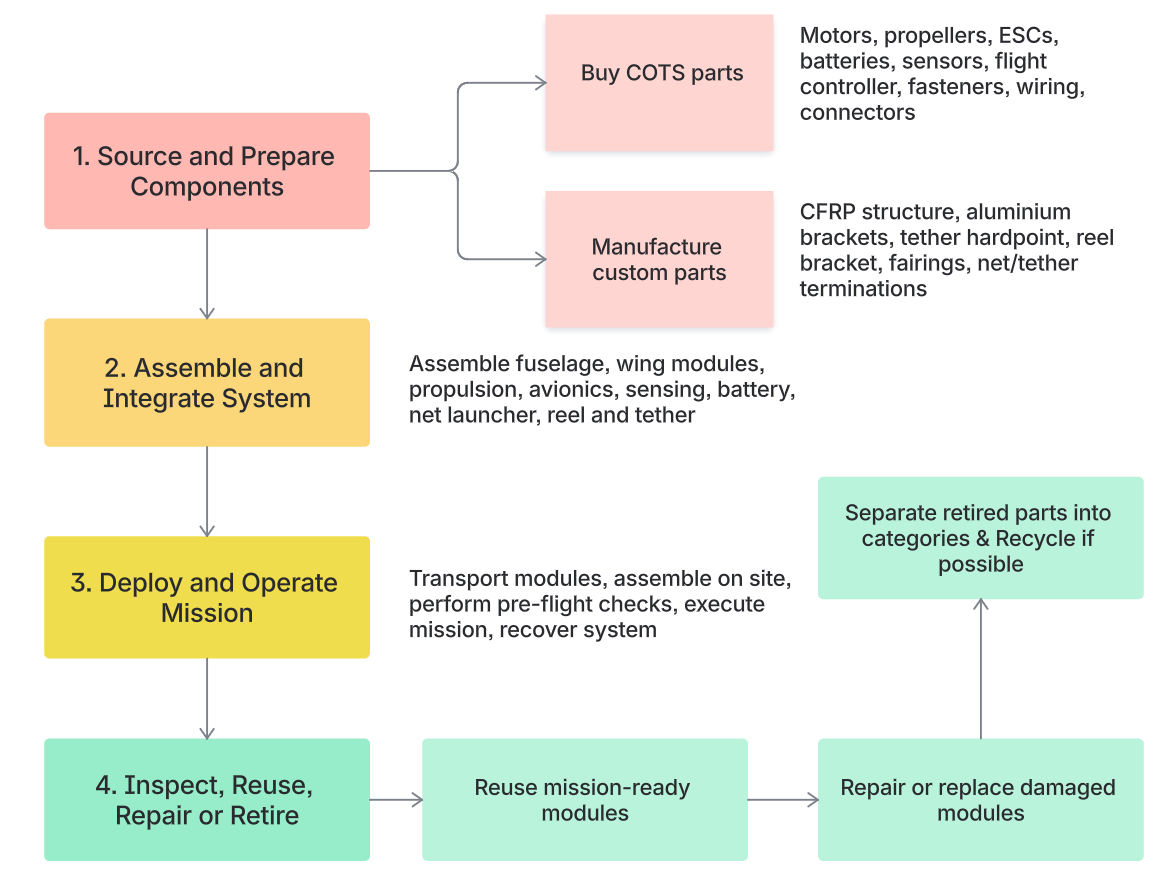
\includegraphics[width=0.60\textwidth]{figures/image.png}
    \caption{Simplified manufacturing, deployment, and life-cycle flow for Concept A.}
    \label{fig:concept_a_lifecycle_flow}
    \vspace{-1em}
\end{wrapfigure}


Figure~\ref{fig:concept_a_lifecycle_flow} summarises the manufacturing and life-cycle logic for Concept A. The process is divided into four main phases: sourcing and preparation, system assembly and integration, mission deployment and operation, and post-mission inspection. Standard components are bought as COTS parts where possible, while mission-specific structural and interaction components are manufactured or prepared separately. After each mission, the recovered system is inspected and either reused, repaired, or separated into end-of-life streams.
The assembly starts with the main airframe. This includes the fuselage frame, lifting surfaces, motor mounts, and landing supports.  Second, the propulsion system, battery and avionics bay are installed while checking centre-of-gravity limits and access to electrical interfaces. Third, the sensing system is mounted and aligned so that its field of view is not blocked by the interaction mechanism or the structure. Fourth, the balloon interaction subsystem is attached to reinforced hardpoint in the nose of the aircraft and checked for deployment clearance. Finally, the complete system is inspected for cable routing, fastener access, propeller clearance, and general maintainability.



This approach reduces the risk that the entire airframe must be replaced after local damage. The most highly loaded and mission-specific components, especially the tether hardpoint, tether, reel bracket and net, should remain inspectable and replaceable.




% \subsection{Main Risks and Final Design Work}


% The final design phase should refine the following items:
% \begin{itemize}
%     \item define the maximum expected tether and capture loads;
%     \item size the tether hardpoint, reel mount, and central fuselage load path;
%     \item update the mass and centre-of-gravity budget;
%     \item check motor mount stiffness and vibration behaviour;
%     \item define the material properties used for structural sizing;
%     \item verify propeller, sensor, and interaction mechanism clearances;
%     \item define inspection and replacement procedures for damaged or worn components.
% \end{itemize}

% \begin{table}[H]
% \centering
% \small
% \caption{Preliminary structural load cases for Concept A.}
% \label{tab:concept_a_structural_load_cases}
% \begin{tabularx}{\textwidth}{p{0.12\textwidth} p{0.32\textwidth} X}
% \toprule
% \textbf{Load case} & \textbf{Description} & \textbf{Critical elements} \\
% \midrule
% LC1 & Hover and climb at maximum take-off mass & Motor mounts, boom roots, central fuselage frame, battery support. \\
% LC2 & Transition between hover and cruise & Wing roots, canard attachments, fuselage torsion path, control surfaces. \\
% LC3 & Net-launcher recoil & Nose frame, launcher mount, local fuselage reinforcement. \\
% LC4 & Maximum tether tension after capture & Tether hardpoint, reel mount, central frame, load-spreading fittings. \\
% LC5 & Emergency breakaway or parachute deployment & Breakaway device, tether attachment, parachute bridle, backup load path. \\
% LC6 & Landing after recovery & Landing supports, lower fuselage frame, battery restraint, propeller clearance. \\
% LC7 & Propulsion vibration and repeated missions & Motor brackets, bolted joints, composite-metal interfaces, avionics mounts. \\
% \bottomrule
% \end{tabularx}
% \end{table}




% \begin{table}[H]
% \centering
% \small
% \caption{Preliminary material allocation for Concept A.}
% \label{tab:concept_a_material_allocation}
% \begin{tabularx}{\textwidth}{p{0.24\textwidth} p{0.23\textwidth} X}
% \toprule
% \textbf{Component} & \textbf{Baseline material} & \textbf{Reason for selection} \\
% \midrule
% Wing, canard, and main frame members & CFRP tubes/plates & High specific stiffness and low mass for the mass-sensitive tail-sitter platform. \\
% Motor mounts and local brackets & Aluminium alloy & Good local load transfer, machinability, inspection access, and replacement after damage. \\
% Central battery bay and fuselage frame & CFRP with local metallic inserts & Lightweight primary structure with reinforced load introduction points. \\
% Tether hardpoint and reel bracket & Aluminium alloy / metallic fitting & Concentrated capture loads require a robust, inspectable, and replaceable interface. \\
% Net and tether & UHMWPE/HMPE fibre & High tensile strength at low mass, flexible deployment, and reuse after nominal missions. \\
% Launcher and sensor fairings & Lightweight polymer or composite & Non-primary parts used for protection and aerodynamic shaping. \\
% Emergency parachute & Ripstop nylon or equivalent fabric & Lightweight, packable, and suitable for emergency descent control. \\


% \bottomrule
% \end{tabularx}
% \end{table}




\section{Balloon Interaction Mechanism}
This subsection will perform a preliminary design of the balloon interaction mechanism. The UAV approaches the suspended payload from below, deploys a net around it, and then uses a tethered connection to guide the balloon and its payload to a recovery zone.
The subsystem is divided into five main elements: the capture net, the net launcher, the tether, the powered reel, and the parachute-based backup system.
A sketch of the net can be found in \autoref{fig:PayloadCapture}.
\begin{figure}[H]
    \centering
    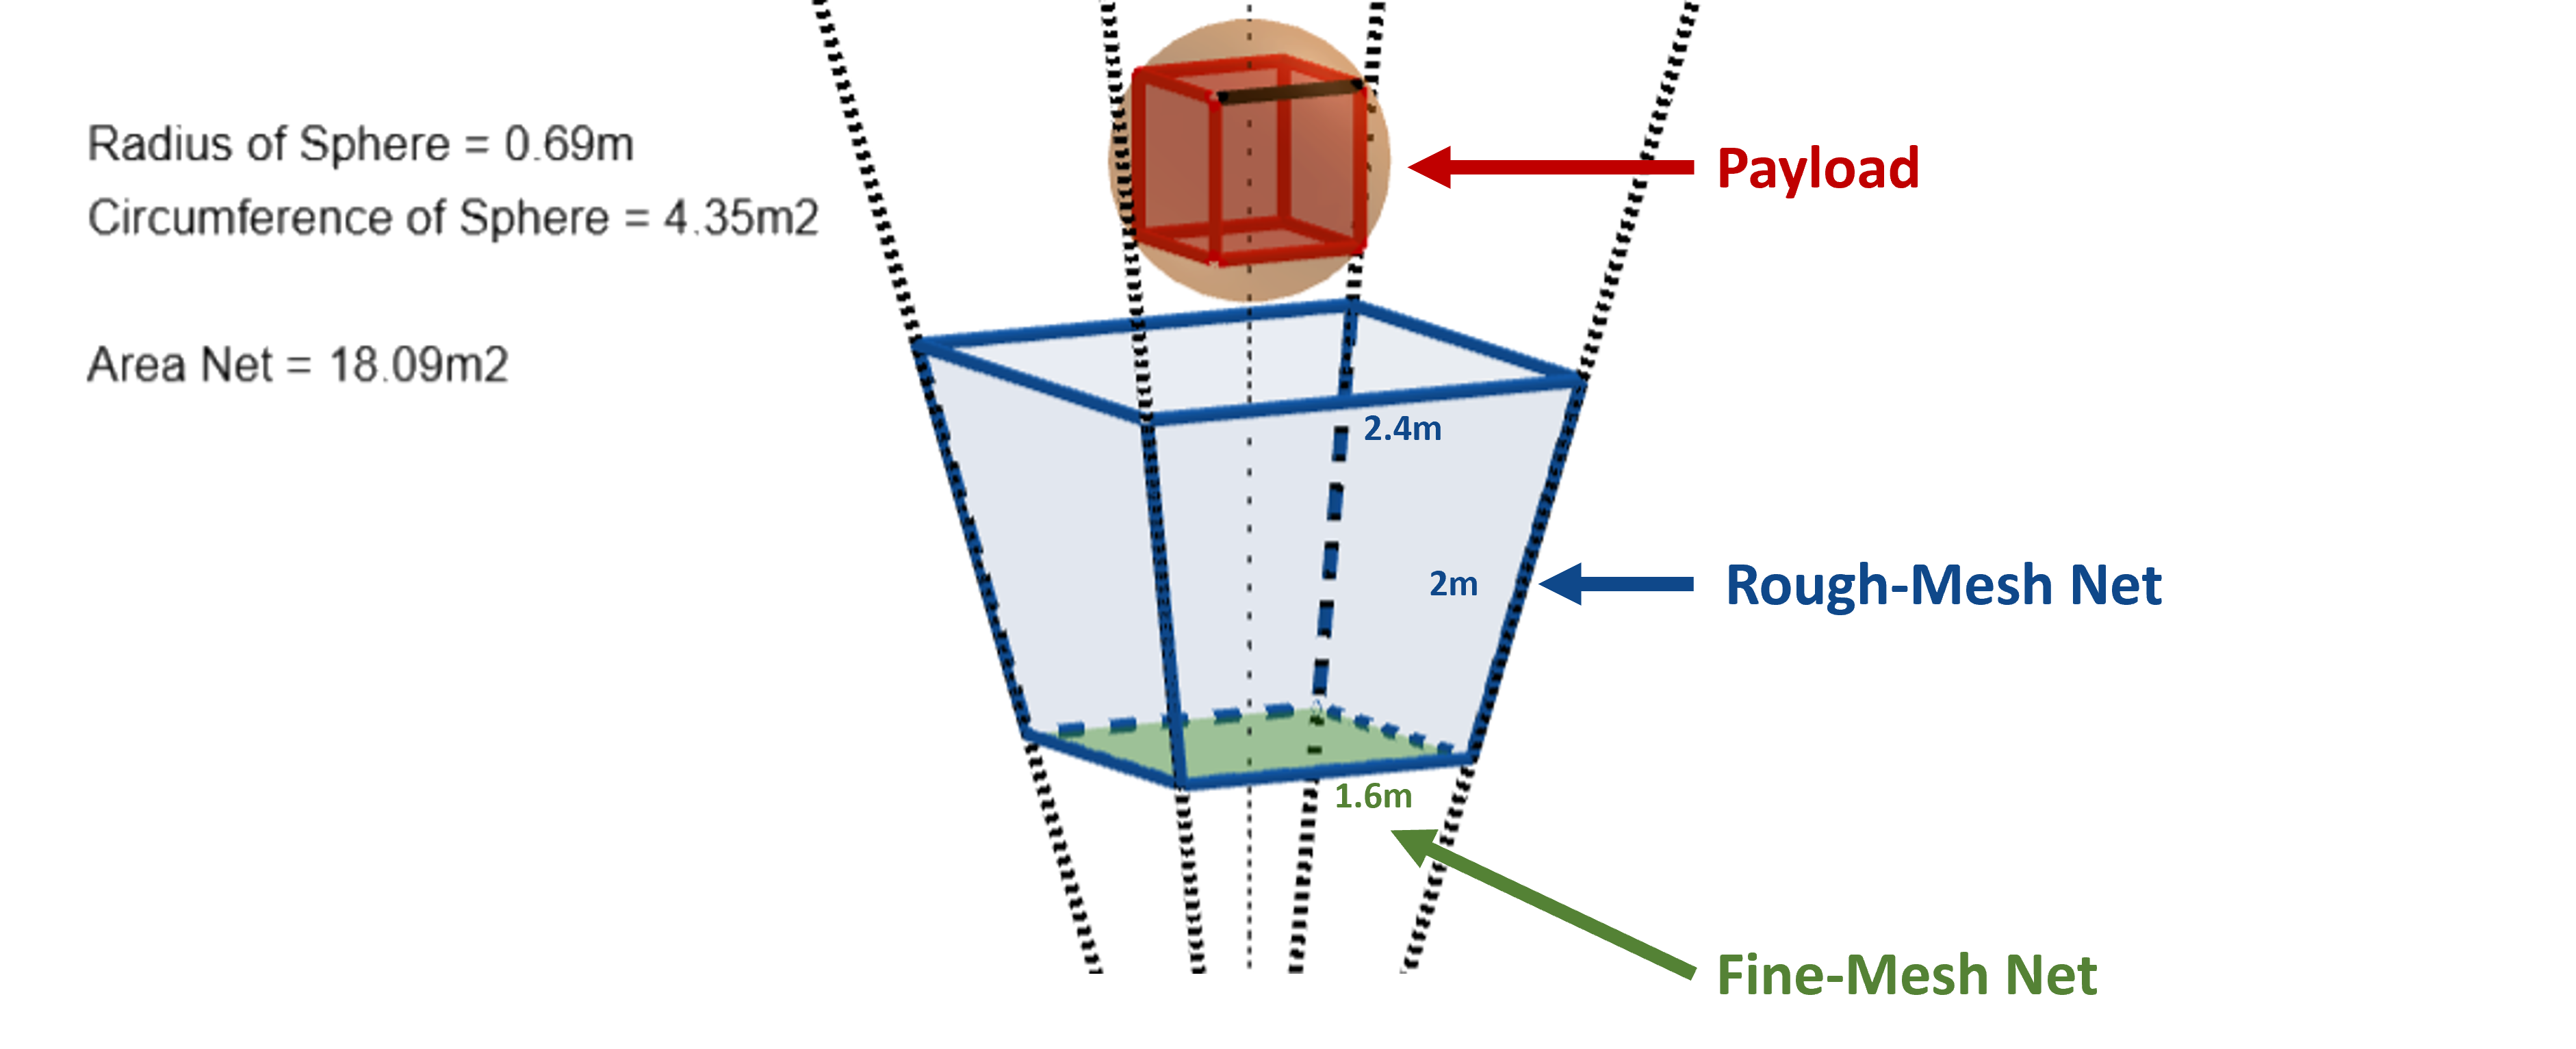
\includegraphics[width=0.8\linewidth]{figures/Payload Capture2.png}
    \caption{Sketch of the Payload Capture}
    \label{fig:PayloadCapture}
\end{figure}



\subsection{Required Net Size}
To start the sizing of the net, a more detailed analysis of payload sizes was performed. \autoref{tab:PayloadDimension} gives an overview of different balloons with their respective payload weights and an upper limit for their dimensions.

\begin{table}[H]
\centering
\small
\caption{Relevant balloons with payload weights and dimensions.}
\label{tab:PayloadDimension}
\begin{tabularx}{\textwidth}{p{0.12\textwidth} p{0.26\textwidth} p{0.15\textwidth} p{0.14\textwidth} p{0.18\textwidth} X}
\toprule
\textbf{Class} & \textbf{Example} & \textbf{Balloon dimensions [m]} & \textbf{Payload mass range [kg]} & \textbf{Payload size range [m $\times$ m $\times$ m]} & \textbf{Source} \\
\midrule

Small & Meteorological radiosonde 
& 2-3 
& 0.1-0.9 
& 0.4 $\times$ 0.3 $\times$ 0.1 
& \\

Medium & Amateur high-altitude 
& 3-4 
& 1-5 
& 0.5 $\times$ 0.5 $\times$ 0.5 
& \\

Large & Smuggling 
& 4-6 
& 10-50 
& 0.8 $\times$ 0.8 $\times$ 0.8 
& \\

\bottomrule
\end{tabularx}
\end{table}

While there are balloons that can carry larger payloads, such as the NASA Super Pressure Balloon\cite{NASA2022Super-pressure-balloon-fact-sheet}, these fall outside of the scope of this project. All relevant payloads within the project scope are therefore assumed to fit inside a 0.8 m cube. To account for non-cubic shapes or protruding antennae, this cube is enclosed by a sphere with a radius of 0.7 m, as illustrated in \autoref{fig:PayloadCapture}

\subsection{Preliminary Net Design}
Now that a new payload size envelope has been defined, the net must be sized accordingly. The UAV has an assumed preliminary estimate of lateral hover accuracy at 6 km altitude of $\pm$50 cm. Thus, a 70 cm radius sphere requires the net opening to be at least 2.4 m. The net has a trapezoidal shape, with the 1.6 m bottom part being slightly larger than the largest assumed payload width of 1.4 m. This is visualized in \autoref{fig:PayloadCapture}.

Since the net has to be launched from the UAV and then must be strong enough to drag the payload, the main drivers are low mass, high tensile strength, abrasion resistance, environmental resistance, and safe interaction with the payload. Nylon is inexpensive and tough, but absorbs moisture, making its performance less predictable in wet conditions. Polyester has better moisture resistance, but a much lower strength-to-weight ratio, while aramid fibers are strong but denser and less favorable for repeated outdoor bending and abrasion. Ultra-high molecular weight polyethylene (UHMWPE) is therefore selected, as it combines very low density with high tensile strength, abrasion resistance, UV stability and negligible water absorption.

The mesh spacing is important, as it strongly influences aerodynamic drag, net mass, and reliability. A fine mesh is required near the bottom of the net, to ensure reliable capture even of smaller payloads. A preliminary bottom mesh spacing of 10 cm is therefore selected. The side mesh may be coarser, with a preliminary spacing of 50 cm.

To ensure that the net securely captures the payload, a pouch-like closing mechanism is used, similar in function to a slip knot. The tether is directly connected to this closing mechanism so that, when the tether is pulled, the top of the net closes. The closing mechanism can therefore be sized by taking the perimeter length of the net and assuming the same material as the tether, as defined below.

When sizing the net, the effects of air resistance and potential energy must be balanced to ensure that the net can be launched upwards as efficiently as possible. \autoref{fig:energyvsmass} shows the relationship between these two considered sources of energy loss. From the figure, it is clear that two criteria drive the choice of net mass: drag, the effect of which decreases with increasing inertia, and required potential energy, which increases with weight. This is because at low masses, assuming constant area, the drag has a larger effect relative to the mass of the net and thus slows it down more, requiring a higher launch velocity. 


The acceptable net assembly mass lies between 550 g and 1.11 kg, corresponding to the range in which the minimum required energy remains within 106 J $\pm 7.5\%$. Adding the estimated masses of the individual components, detailed in \autoref{tab:NetAssemblyMass}, yields 570 g, falling within this range. This requires a minimum amount of energy to reach the altitude and counteract drag of 112 J. 

\begin{figure}[H]
    \centering
    % --- LEFT SIDE: FIGURE (Aligned at top) ---
    \begin{minipage}[t]{0.48\textwidth}
        \vspace{0pt} % Sets a top anchor point
        \centering
        \raisebox{-\height}{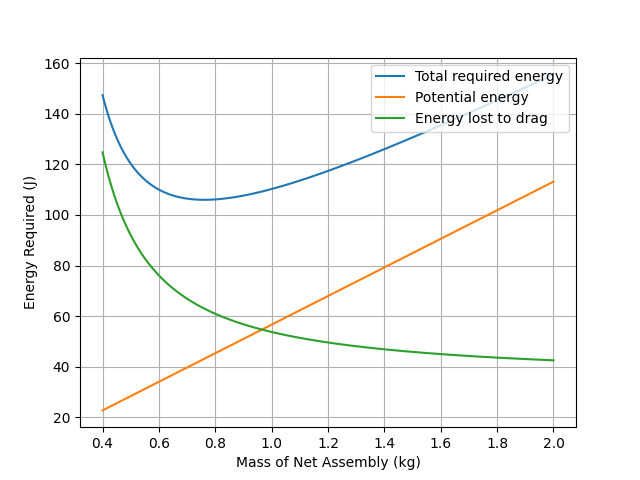
\includegraphics[width=\linewidth]{figures/EnergyvsMass.png}}
        \caption{Theoretical Required Energy vs Mass of Net Assembly}
        \label{fig:energyvsmass}
    \end{minipage}%
    \hfill
    % --- RIGHT SIDE: TABLE (Aligned at top) ---
    \begin{minipage}[t]{0.48\textwidth}
        \vspace{1cm} % Sets a top anchor point
        \centering
        \captionof{table}{Mass of Net Assembly Split by Component}
        \label{tab:NetAssemblyMass}
        \vspace{6pt}
        \footnotesize
        \begin{tabular}{ll}
        \hline
        \textbf{Component}          & \textbf{Estimated Mass [g]} \\ \hline
        Net                         & 150                          \\
        Corner Weights              & 75 $\times$ 4 (300 total)    \\
        Closing Mechanism           & 100                          \\
        Tether                      & 20                           \\ \hline
        \textbf{Total Net Assembly} & 570                          \\ \hline
        \end{tabular}
    \end{minipage}
\end{figure}



\subsection{Preliminary Net Launcher Design}
The net launcher is required to deploy the net, weights and tether upwards with sufficient height margin to reliably envelop the full payload, including an assumed vertical positioning uncertainty of approximately 0.5 m. This yields a required shooting height of just under 6 m. Several concepts were considered, including CO\textsubscript{2} cartridges, compressed-air storage, springs, electromagnetic launchers, and powered weights.

For preliminary sizing, the launch height requirement was converted into an initial velocity requirement, resulting in a minimum stored energy of approximately 480 J. This includes a safety factor of 4 to account for uncertainties such as energy losses during net unfolding. This results in a target launch speed of at least 20 m/s.

Based on comparable net launchers, such as the one in \autoref{fig:exnetlauncher}, a compressed-gas launcher is selected as the preliminary option. CO\textsubscript{2} or compressed-air actuation can provide the required stored energy while remaining consistent with the non-explosive and non-pyrotechnic requirement. The pneumatic system is less compact than cartridge-based launchers, so the pressure vessel, valve and barrel geometry must be refined during detailed design to confirm mass, packaging and repeatability margins.

\begin{figure}[H]
    \centering 
    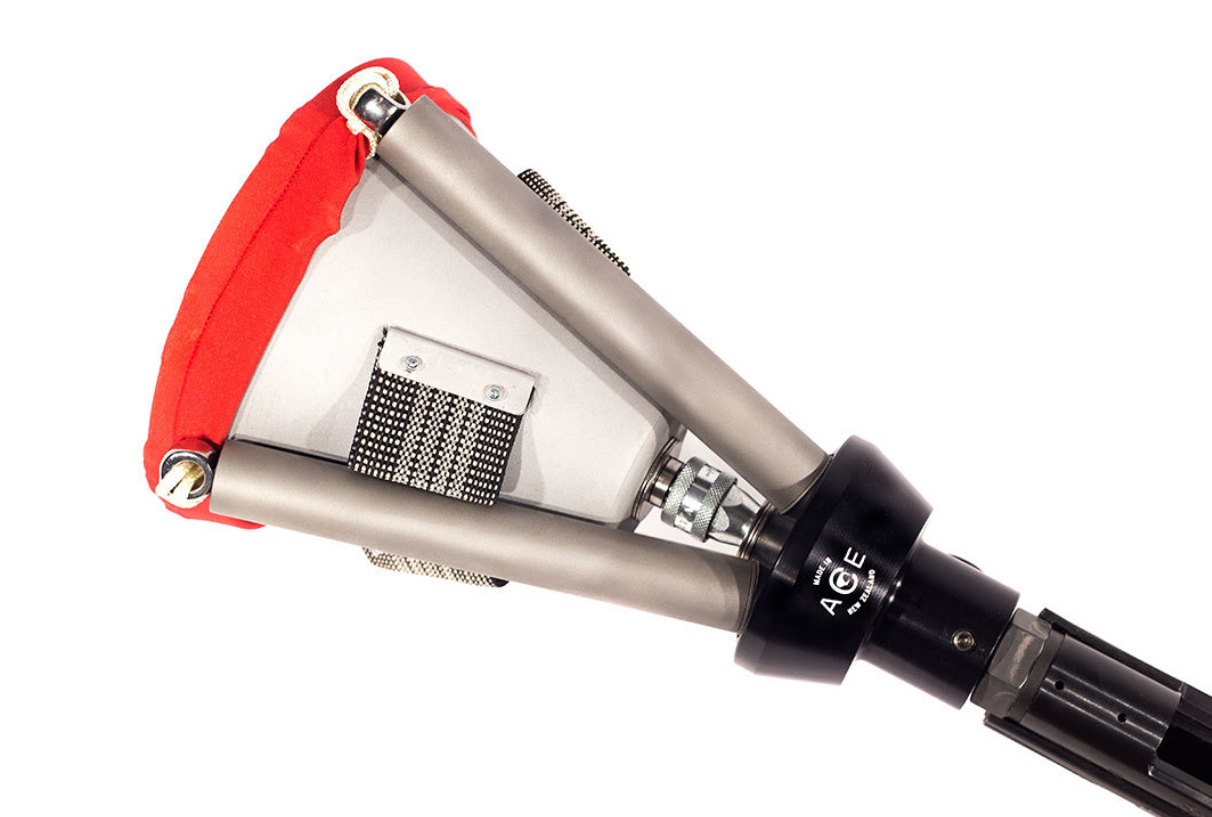
\includegraphics[width=0.3\linewidth]{figures/Net Gun.png}
    \caption{Similar Net Launcher\cite{netgun.comUltraNet-HDGun}}
    \label{fig:exnetlauncher}
\end{figure}


\subsection{Preliminary Tether Design}
For the tether connecting the UAV and the net, UHMWPE is also selected for its very high strength-to-weight ratio. The tether is sized for an estimated maximum balloon drag load of approximately 1000 N, with a safety factor of 4 accounting for shock and dynamic loads. A 2 mm braided UHMWPE line is suitable as a preliminary choice, having a breaking load of about 4 kN while maintaining a very low weight.

The tether length is set to 25 m, consisting of a 20 m nominal separation distance between UAV and net plus 5 m to give margin in case the tether unravels slightly.

The tether should be attached to the UAV close to the center of gravity to minimize moments while dragging the balloon and captured payload to the recovery zone. Depending on the final configuration and propeller position, a line guide may also be included to prevent tangling.

\subsection{Preliminary Reel Design}
The tether is connected to the UAV with a powered reel. This allows adjusting the distance between the balloon and the UAV, while also providing shock-load protection by rolling out the tether during sudden load spikes.

A preliminary drum core diameter of 40 mm gives a core circumference of approximately 0.125 m, requiring about 200 turns to store the full 25 m tether at the core diameter. With a 100 mm drum width, approximately 50 turns of 2 mm tether fit per layer. The drum is thus sized for 6 layers (including two layers of margin), increasing the effective radius to a worst-case value of approximately 32 mm.

To prevent direct shock transfer to the UAV, the reel should include an adjustable disk-based drag stack, set to avoid uncontrolled unspooling but low enough to slip under peak capture loads. Since the motor only needs to retract the tether and not continuously pull the full balloon load, a design pull load of 250 N is used, requiring a drum torque of about 8 Nm. Retraction at 1 m/s corresponds to an ideal mechanical power of approximately 250 W. Therefore, a lightweight brushless motor with a roughly 10:1 gear reduction is suitable for this application.

\subsection{Preliminary Parachute Design}
A parachute is included as a safety system in case the balloon bursts and the captured payload, with a mass up to 50 kg, enters free fall. In this case, the payload is separated from the UAV, preventing the payload from overloading or destabilizing the vehicle.
A 15 m\textsuperscript{2} rescue parachute for UAV applications is rated for payloads in this range and has a mass of approximately 600 g, making it feasible to integrate without a large mass penalty. Deployment can be triggered mechanically by a shear pin under excessive tether load, or by reaching the end of the reel travel, depending on the final mechanism design.

\section{Operations, Ground System \& Safety}

This section presents the preliminary evaluation of the UAV ground system, operational concept, and associated safety provisions. The ground system is responsible for supporting the tail-sitter UAV before, during, and after a mission by providing the infrastructure required for storage, launch preparation, recovery, charging, inspection, and safe standby operation. Since the UAV is intended to operate in an airport environment, the ground system must also interface with operational approval procedures, restrict unauthorised access, and support safe contingency handling.

%The ground system is not treated as a passive support element, but as part of the overall mission architecture. For a tail-sitter UAV, repeatable launch and recovery conditions are especially important because the aircraft transitions between vertical ground handling and airborne operation. Therefore, the selected ground system must provide a stable launch and recovery interface, reliable communication support, controlled battery handling, and a clear post-mission turnaround procedure. These functions directly influence operational reliability, safety, and deployment feasibility.

Based on the Ground System, Operations, and Safety design option trees, three representative concepts were selected for comparison. These concepts are summarised in \autoref{tab:UAVConcepts}. The concepts were evaluated in \autoref{tab:ground_system_tradeoff} using criteria that reflect the most important operational and implementation drivers for airport deployment. Cost, reliability, servicing and availability, safety, flexibility, scalability, and complexity were included because they determine whether the ground system can be deployed, operated, maintained, and expanded in a practical way.

The criteria were weighted according to their importance at this stage of the design. Cost, reliability, and safety were assigned the highest weights because they strongly affect the feasibility and acceptability of the ground system. Servicing and availability, flexibility, and complexity were given medium weights because they influence day-to-day operation and integration effort, while scalability was given a lower weight because large-scale deployment is less critical than proving a robust baseline architecture at the preliminary design stage.





{
\small
\setlength{\LTleft}{0pt}
\setlength{\LTright}{0pt}

\begin{longtable}{@{}
>{\raggedright\arraybackslash}p{0.15\textwidth}
>{\raggedright\arraybackslash}p{0.28\textwidth}
>{\raggedright\arraybackslash}p{0.27\textwidth}
>{\raggedright\arraybackslash}p{0.25\textwidth}
@{}}
\caption{Architectural and Operational Concept Profiles for the UAV Ground System.}
\label{tab:UAVConcepts} \\
\toprule
\textbf{Concept} & \textbf{Ground System} & \textbf{Operations} & \textbf{Safety \& Contingency} \\
\midrule
\endfirsthead

\toprule
\textbf{Concept} & \textbf{Ground System} & \textbf{Operations} & \textbf{Safety \& Contingency} \\
\midrule
\endhead

\bottomrule
\endfoot

Concept 1 & 
Container-based station with slide-out platform, automated clamps, and directional tracking antenna. & 
ATC-gated remote approval, human-in-the-loop, and post-mission manual inspection. & 
Fire-isolated charging cabinet, access-controlled enclosure, and land at nearest safe zone. \\
\addlinespace

Concept 2 & 
Truck-mounted station, covered deck, and manual/automatic battery swap. & 
ATC-gated launch interlock, remote approval, and automatic recharge with health check. & 
Perimeter safety fencing, maintenance lockout system, and automatic flight termination. \\
\addlinespace

Concept 3 & 
Off-grid solar-powered station with autonomous robotic battery hot-swapping and open outdoor deck. & 
Fully autonomous network dispatch, authority-gated routing, and automated recovery cycle. & 
Onboard ballistic emergency parachute deployment and automated vehicle termination. \\

\end{longtable}
}

{
\tiny
\setlength{\LTleft}{0pt}
\setlength{\LTright}{0pt}
\setlength{\tabcolsep}{1.4pt}
\renewcommand{\arraystretch}{0.92} % Tightens row padding baseline
% Swapped inner \tiny to \scriptsize so it scales gracefully with global \tiny block
\newcommand{\gscell}[3]{\cellcolor{#1}\makecell{\textbf{#2}\\[-0.2ex]\scriptsize #3}} 

\begin{longtable}{|
    >{\raggedright\arraybackslash}p{0.31\textwidth}|
    >{\centering\arraybackslash}p{0.21\textwidth}|
    >{\centering\arraybackslash}p{0.21\textwidth}|
    >{\centering\arraybackslash}p{0.21\textwidth}|
}
\caption{Ground system concept trade-off.}
\label{tab:ground_system_tradeoff} \\
\hline
\diagbox[
    width=\dimexpr0.31\textwidth+2\tabcolsep+2\arrayrulewidth\relax,
    height=0.035\textwidth, % Squeezed header box height
    innerleftsep=0.002\textwidth,
    innerrightsep=0.002\textwidth
]{\textbf{Criteria}}{\shortstack[r]{\textbf{Concepts}}}
& \makecell{\textbf{Concept}\\\textbf{1}}
& \makecell{\textbf{Concept}\\\textbf{2}}
& \makecell{\textbf{Concept}\\\textbf{3}}
\\ \hline
\endfirsthead

\hline
\diagbox[
    width=\dimexpr0.31\textwidth+2\tabcolsep+2\arrayrulewidth\relax,
    height=0.035\textwidth,
    innerleftsep=0.002\textwidth,
    innerrightsep=0.002\textwidth
]{\textbf{Criteria}}{\shortstack[r]{\textbf{Concepts}}}
& \makecell{\textbf{Concept}\\\textbf{1}}
& \makecell{\textbf{Concept}\\\textbf{2}}
& \makecell{\textbf{Concept}\\\textbf{3}}
\\ \hline
\endhead

\hline
\endfoot

% Removed all \rule spacing commands
\makecell[l]{\textbf{Screening}\\\textbf{outcome}}
& \gscell{blue!30}{Retain}{best overall\\score; balanced\\ground system}
& \gscell{yellow!40}{Backup}{high mobility;\\lower reliability\\and safety}
& \gscell{yellow!40}{Backup}{safe and\\available; low\\flexibility}
\\ \hline

\makecell[l]{\textbf{Cost}\\\textbf{3}}
& \gscell{yellow!40}{3.0}{moderate\\station, service\\and deployment cost}
& \gscell{yellow!40}{3.0}{low deployment\\cost; higher\\manual upkeep}
& \gscell{yellow!40}{2.7}{fixed works\\increase install\\and manufacturing}
\\ \hline

\makecell[l]{\textbf{Reliability}\\\textbf{3}}
& \gscell{blue!30}{4.0}{directional\\tracking link;\\stable deployment}
& \gscell{orange!40}{2.5}{mobile setup;\\weaker link and\\deployment repeatability}
& \gscell{blue!30}{4.0}{fixed setup;\\airport network\\interface}
\\ \hline

\makecell[l]{\textbf{Servicing}\\\textbf{and availability 2}}
& \gscell{blue!30}{3.7}{same-station\\return; manual\\inspection remains}
& \gscell{yellow!40}{2.7}{more crew;\\manual recovery\\and reset}
& \gscell{blue!30}{4.0}{automatic\\checks; fast\\return to standby}
\\ \hline

\makecell[l]{\textbf{Safety}\\\textbf{3}}
& \gscell{blue!30}{3.8}{controlled bay;\\ATC-gated;\\safe abort}
& \gscell{yellow!40}{3.0}{mobile site;\\higher ground\\crew exposure}
& \gscell{blue!30}{3.8}{strong ATC\\integration; lower\\battery safety}
\\ \hline

\makecell[l]{\textbf{Flexibility}\\\textbf{2}}
& \gscell{yellow!40}{3.0}{relocatable;\\still container\\dependent}
& \gscell{green!40}{4.7}{high mobility;\\adaptable to\\different sites}
& \gscell{orange!40}{2.0}{fixed site;\\low deployment\\mobility}
\\ \hline

\makecell[l]{\textbf{Scalability}\\\textbf{1}}
& \gscell{blue!30}{3.8}{repeatable\\container units;\\modular growth}
& \gscell{blue!30}{4.0}{mobile units\\increase coverage\\quickly}
& \gscell{yellow!40}{2.8}{each location\\needs airport\\integration}
\\ \hline

\makecell[l]{\textbf{Complexity}\\\textbf{2}}
& \gscell{yellow!40}{3.0}{moderate\\automation and\\infrastructure}
& \gscell{yellow!40}{3.0}{simple install;\\more manual\\operation}
& \gscell{yellow!40}{2.8}{fixed infrastructure\\and integration\\increase complexity}
\\ \hline

\makecell[l]{\textbf{Weighted}\\\textbf{score/rank}}
& \cellcolor{blue!30}\makecell{\textbf{3.50}\\\textbf{1}}
& \cellcolor{yellow!40}\makecell{\textbf{3.10}\\\textbf{3}}
& \cellcolor{yellow!40}\makecell{\textbf{3.20}\\\textbf{2}}
\\ \hline

\end{longtable}

\vspace{-0.5cm} % Squeezes spacing between the table and the legend color bar

\begin{center}
\tiny % Dropped from \scriptsize to maintain unified document flow
\renewcommand{\arraystretch}{0.85}
\setlength{\tabcolsep}{3pt}
\begin{tabular}{|l|l|l|l|l|}
\hline
\cellcolor{green!40} 5: Excellent &
\cellcolor{blue!30} 4: Good &
\cellcolor{yellow!40} 3: Fair &
\cellcolor{orange!40} 2: Poor &
\cellcolor{red!40} 1: Unacceptable \\
\hline
\end{tabular}
\end{center}
}

%Based on the concept description and trade-off analysis, Concept 1 was selected as the preliminary architecture for the UAV ground system. It achieves the highest weighted score, with a final score of $3.50$, because it provides the best balance between operational reliability, safety, and deployability. The container-based station gives the tail-sitter UAV a repeatable and protected operating environment, while the slide-out platform, automated clamps, and directional tracking antenna reduce uncertainty during launch, recovery, and communication.

%The main advantage of Concept 1 over Concept 2 is operational repeatability. Although Concept 2 offers the highest flexibility due to its truck-mounted configuration, this mobility also introduces more variation between operating locations. Each deployment may differ in ground conditions, antenna placement, vehicle levelling, crew access, and safety perimeter control. These variations make the launch and recovery process less predictable, which explains the lower reliability score assigned to Concept 2. Concept 1 avoids this issue by using a more stable station architecture while still remaining relocatable if airport layout or mission requirements change.

%Concept 3 performs well in availability and automation because robotic battery swapping, autonomous checks, and fixed infrastructure could allow faster return to standby. However, this benefit comes with reduced flexibility and higher site-dependency. Since each deployment location would require more permanent airport integration and fixed infrastructure, Concept 3 is less suitable for a preliminary architecture that must remain adaptable to different airport layouts and operational constraints. Its strong automation potential therefore does not fully compensate for its lower flexibility, higher installation effort, and increased integration complexity.

%Concept 1 was therefore retained because it forms a practical intermediate solution between the mobile truck-based concept and the fully fixed autonomous network concept. It provides a controlled and access-limited ground station, supports ATC-gated operation, protects the charging process through fire-isolated containment, and still allows manual post-mission inspection before the UAV is returned to service. This makes it a suitable baseline for further development of the ground system and operational concept.

Based on the trade-off analysis, Concept 1 was selected as the preliminary ground system architecture because its container-based design achieves the highest weighted score (3.50) by optimizing the balance between operational reliability, safety, and deployability. While Concept 2 offers high flexibility through its truck-mounted configuration, it suffers from poor operational repeatability and lower reliability due to unpredictable site-by-site variations. Conversely, Concept 3 delivers excellent automation and availability via robotic battery swapping, but its high infrastructure complexity and rigid site-dependency drastically limit its deployment flexibility. Ultimately, Concept 1 provides the ideal intermediate solution—delivering a standardized, stable, and risk-averse environment with strong ATC integration and balanced lifecycle costs, making it the most robust foundation for subsequent design phases.


\subsection{Selected Ground System Architecture}

The selected ground system consists of a container-based station with an integrated slide-out platform, automated holding clamps, fire-isolated charging cabinet, access-controlled enclosure, and directional tracking antenna. The container provides a protected environment for storage and servicing, while the slide-out platform creates a repeatable interface for launch and recovery. The automated clamps are included to secure the UAV during standby, pre-flight preparation, and post-landing handling, reducing the dependence on manual intervention near the aircraft.
\\
The directional tracking antenna is included to improve communication robustness during the mission. Since the station geometry is fixed relative to the launch and recovery platform, the antenna can be installed and aligned in a repeatable way. This is preferable to a mobile or temporary setup, where antenna placement may depend on the specific deployment location and available ground space. The selected architecture therefore supports both communication reliability and operational consistency.
\\
The fire-isolated charging cabinet is included because battery charging is one of the main ground-based safety concerns. By separating charging from the main access area and enclosing it in a dedicated protected compartment, the consequences of a battery-related incident can be reduced. This also allows charging procedures, battery inspection, and ground-crew access to be controlled more clearly than in an exposed or improvised setup.





% % \section{RAMS Characteristics}

% % This section presents a preliminary Reliability, Availability, Maintainability, and Safety (RAMS) assessment of the selected BELLONA system. At this stage, the RAMS assessment is mainly qualitative, because detailed component failure rates, repair times, and operational downtime data are not yet available. The purpose of this section is therefore to identify the main design features that support dependable operation, as well as the remaining RAMS drivers that must be verified in the next design phase.

% % \textbf{Reliability} is supported by the single-UAV architecture of Concept A. Compared with multi-UAV concepts, the selected tail-sitter avoids cooperative formation control, inter-vehicle coordination, and multi-vehicle sequencing during capture. This reduces the number of mission-critical dependencies. However, the selected concept still contains several reliability-critical phases: tail-sitter transition, hover below the payload, upward net deployment, net closure, tether-load control, and post-capture descent. The most important reliability drivers are therefore the terminal sensing chain, the net-launch mechanism, the tether reel, and the flight controller's ability to remain stable after the payload is captured. To improve reliability, the system uses external target cueing, onboard terminal sensing, tether-load feedback, and mission decision gates before launch, capture, and descent. These measures reduce the probability of continuing the mission when tracking quality, energy margin, or capture geometry is insufficient.

% % \textbf{Availability} describes whether the system is ready to perform a mission when required. For BELLONA, availability is driven by battery state, weather conditions, target cue quality, system health, recovery-zone availability, and post-mission turnaround time. The selected ground system supports availability by combining storage, launch preparation, charging, inspection, and communication support in one controlled station. After a mission, the UAV can return to the station for inspection, battery charging, net replacement, and tether/reel checks. Manual inspection is still required because the balloon-interaction mission may introduce unusual loads, payload contact, soft-goods wear, or minor structural damage. Although this reduces turnaround speed compared with a fully automated system, it improves confidence that the UAV is not returned to standby in a damaged state.

% % \textbf{Maintainability} is addressed through modularity and accessibility. The aircraft architecture should allow high-wear or mission-exposed components to be inspected and replaced without disturbing the full airframe. This is especially important for the net, tether, closure line, corner weights, reel, hardpoints, propeller guards, landing supports, and battery system. The structural concept should therefore include accessible hardpoints, inspectable metallic fittings, removable wing or fuselage modules where practical, and replaceable soft-goods elements. The ground station also supports maintainability by providing a defined location for charging, inspection, safe handling, and storage. In the next design phase, maintainability must be strengthened by defining inspection intervals, replacement limits for the net and tether, access requirements for the reel and battery system, and proof-load checks for the capture load path.

% % \textbf{Safety} is one of the main reasons for selecting Concept A. The system captures the suspended payload from below and avoids intentional balloon destruction, which reduces the risk of uncontrolled deflation, falling debris, and damage to the payload. During the mission, safety is controlled through decision gates: pre-flight approval, target confirmation, sufficient energy margin, acceptable tracking quality, safe interaction geometry, recovery-zone availability, and abort availability. After capture, the powered reel and tether-load monitoring help manage the coupled UAV--balloon--payload system during descent. If the balloon ruptures, the tether load becomes unsafe, or the payload begins to fall uncontrollably, an emergency separation system is required so that the UAV can disconnect from the payload-net system. A backup parachute or drag device can then reduce the descent risk of the released payload-net bundle.

% % The main residual safety concerns are net or tether interference with the propellers, partial capture, excessive payload swing, loss of target tracking, and insufficient towing authority in wind. These risks are consistent with the updated risk register and therefore require focused verification. The next design phase should include simulation of tether dynamics, net-clearance checks, ground testing of net deployment repeatability, proof-load testing of the capture load path, hover-alignment tests, captive-load flight tests, and representative balloon-payload interaction trials.

% % Overall, the selected concept provides a strong preliminary RAMS baseline because it avoids the coordination burden of multi-UAV concepts while retaining non-destructive capture and controlled recovery. Its RAMS performance is not yet fully proven, however, because the most critical failure modes are concentrated in the net deployment, tethered-load control, and post-capture descent phases. These items should therefore remain priority verification points during detailed design.

\section{RAMS Characteristics}

This section gives a preliminary qualitative RAMS assessment of Concept A. Since detailed failure rates, repair times, and downtime data are not yet available, the focus is on the main dependability drivers and verification needs.

\textbf{Reliability} is supported by the single-UAV architecture, which avoids the coordination and sequencing risks of multi-UAV concepts. The main reliability-critical phases are tail-sitter transition, hover below the payload, net deployment, net closure, tether-load control, and post-capture descent. Key drivers are therefore terminal sensing, the net launcher, tether reel, and flight-control stability after capture. External cueing, onboard sensing, tether-load feedback, and decision gates reduce the risk of continuing under poor tracking, low energy margin, or unsafe capture geometry.

\textbf{Availability} is driven by battery state, weather, cue quality, system health, recovery-zone availability, and turnaround time. The ground station supports storage, launch preparation, charging, inspection, communication, net replacement, and tether/reel checks. Manual inspection remains necessary after each mission because payload contact, unusual loads, soft-goods wear, or minor structural damage may occur.

\textbf{Maintainability} relies on modular and accessible design. Mission-exposed parts such as the net, tether, closure line, corner weights, reel, hardpoints, propeller guards, landing supports, and battery system should be inspectable and replaceable without major airframe disassembly. The next phase should define inspection intervals, replacement limits, access requirements, and proof-load checks.

\textbf{Safety} is a main reason for selecting Concept A. Capturing the suspended payload from below avoids intentional balloon destruction and reduces the risk of uncontrolled deflation, falling debris, and payload damage. Safety is managed through decision gates for launch, target confirmation, energy margin, tracking quality, interaction geometry, recovery-zone availability, and abort capability. Emergency separation and a backup parachute or drag device are required for balloon rupture, unsafe tether loads, or uncontrolled payload descent.

The main residual risks are net/tether interference with propellers, partial capture, payload swing, loss of tracking, and insufficient towing authority in wind. These should be verified through tether-dynamics simulation, net-clearance checks, net-deployment tests, proof-load tests, hover-alignment tests, captive-load flight tests, and representative balloon-payload trials.
